%
% File ACL2016.tex
%

\documentclass[11pt]{article}

\usepackage{microtype}
\usepackage{acl2016}
\usepackage{url}

% \makeatletter
% \def\url@itstyle{%
%  \@ifundefined{selectfont}{\def\UrlFont{\it}}{\def\UrlFont{\itshape}}}
% \makeatother
% \urlstyle{it}

\makeatletter
\newcommand{\@BIBLABEL}{\@emptybiblabel}
\newcommand{\@emptybiblabel}[1]{}
\makeatother
\interfootnotelinepenalty=10000

\usepackage[hidelinks]{hyperref}

% \usepackage{newtxtext,newtxmath}
\usepackage{times}
\usepackage{color}
\usepackage{enumerate}
\usepackage{amsmath}
\usepackage{amssymb}
\usepackage{amsfonts}
\usepackage{multirow}
\usepackage{latexsym}
\usepackage{array}
\usepackage{tikz}
\usepackage{booktabs}



\aclfinalcopy % Uncomment this line for the final submission
% \def\aclpaperid{***} %  Enter the acl Paper ID here

\newcommand\BibTeX{B{\sc ib}\TeX}

%\title{Towards A Better Understanding on Reading Comprehension}
\title{A Thorough Examination of the \\ CNN\slash Daily Mail Reading Comprehension Task}

\author{Danqi Chen \and Jason Bolton \and Christopher D. Manning\\
            Computer Science
	    Stanford University\\
	    Stanford, CA 94305-9020, USA\\
	    {\tt \{danqi,jebolton,manning\}@cs.stanford.edu}}

\DeclareMathOperator*{\argmin}{arg\,min}
\DeclareMathOperator*{\argmax}{arg\,max}
\DeclareMathOperator*{\sigm}{sigm}
\DeclareMathOperator*{\softmax}{softmax}
\newcommand{\notate}[1]{\textcolor{red}{\textbf{[#1]}}}
\newcommand{\comment}[1]{\textcolor{gray}{\textbf{[#1]}}}
\newcommand{\mf}[1]{\mathbf{#1}}
\newcommand{\tf}[1]{\textbf{#1}}
\newcommand{\ti}[1]{\textit{#1}}
\newcommand{\ttt}[1]{\texttt{#1}}
\newcommand\R{\mathbb{R}}
\newcommand{\specialcell}[2][c]
\newcommand{\finaldm}{76.6\%}

\newcolumntype{C}[1]{>{\centering\let\newline\\\arraybackslash\hspace{0pt}}m{#1}}
\newcommand{\figref}[1]{Figure~\ref{fig:#1}}
\hyphenation{At-ten-tive-Reader}
\hyphenation{Lamb-da-MART}

\renewcommand\floatpagefraction{.9}
\renewcommand\dblfloatpagefraction{.9}
\renewcommand\textfraction{.05}


\date{}

\def\allfiles{}

\begin{document}
\def\tinyweeny{\fontsize{6pt}{8pt}\selectfont}

\maketitle

\begin{abstract}

Enabling a computer to understand a document so that it can answer comprehension questions is a central, yet unsolved goal of NLP\@. A key factor impeding its solution by machine learned systems is the limited availability of human-annotated data. \newcite{hermann2015teaching} seek to solve this problem by creating over a million training examples by pairing \ti{CNN} and \ti{Daily Mail} news articles with their summarized bullet points, and show that a neural network can then be trained to give good performance on this task. In this paper, we conduct a thorough examination of this new reading comprehension task. Our primary aim is to understand what depth of language understanding is required to do well on this task. We approach this from one side by doing a careful hand-analysis of a small subset of the problems and from the other by showing that simple, carefully designed systems can obtain accuracies of {\finalcnn} and {\finaldm} on these two datasets, exceeding current state-of-the-art results by {7}--{10}\%  and approaching what we believe is the ceiling for performance on this task.\footnote{Our code is available at \url{https://github.com/danqi/rc-cnn-dailymail}.}
\end{abstract}


%\cite{burger2001issues}
%\cite{fader2014open}
%\cite{voorhees1999trec}


%A huge leap forward in artificial intelligence will be achieved when
%machines will be able to answer any question expressed in natural
%language. As such, q

Question answering (QA) has been a long standing research problem in
natural language processing, with the first systems attempting to
answer questions by directly reading
documents \citep{voorhees2000building}. The development of large-scale Knowledge Bases (KBs) such as Freebase  \citep{bollacker2008freebase}
helped organize information into structured forms, prompting recent progress to focus on answering questions by converting them into logical forms that can be used to query such databases \citep{berant2013semantic,kwiatkowski-EtAl:2013:EMNLP,fader2014open}.

Unfortunately, KBs have intrinsic limitations such as their inevitable incompleteness and fixed schemas that cannot support all varieties of answers.
%
Since information extraction (IE) \citep{craven2000learning}, intended to
fill in missing information in KBs, is neither accurate nor
reliable enough, collections of raw textual resources and
documents such as Wikipedia will always contain more information.
%than KBs.
%
As a result, even if KBs can be satisfactory for closed-domain problems, they are unlikely
to scale up to answer general questions on any
topic.
%
Starting from this observation,
%here we propose  to study the problem
in this work we study the problem
of answering by directly reading documents.


Retrieving answers directly from text is harder than
from KBs because information is far less structured, is
indirectly and ambiguously expressed, and is usually scattered across multiple documents.
%
%This explains why, when a satisfactory KB is
%available -- which is typically only the case in closed domains --
%using it instead of raw text is preferred. %, because performance is better.
%
This explains why using a satisfactory KB---typically only available in closed domains---is preferred over raw text.
%
We postulate that before trying to provide answers that are not in
KBs, document-based QA systems should first reach KB-based systems'
performance in such closed domains, where clear comparison and
evaluation is possible.
%
To this end, this paper introduces {\sc WikiMovies}, a new
analysis tool that allows for measuring the performance of %loss induced on
QA systems when the knowledge source is switched from a KB to unstructured documents.
%
{\sc WikiMovies} contains $\sim$100k questions in the movie domain, and was designed
to be answerable by using either a perfect KB
(based on OMDb\footnote{\url{http://www.omdbapi.com}}), Wikipedia pages or an imperfect KB obtained through
running %a standard IE pipeline on those pages.
an engineered IE pipeline on those pages.

To bridge the gap between using a KB and reading documents directly,
we still lack appropriate machine learning algorithms. In this
work we propose the Key-Value Memory Network (KV-MemNN), a new neural network
architecture that generalizes the original Memory Network
\citep{sukhbaatar2015end} and can work with either knowledge source.
%
The KV-MemNN performs QA by first storing facts in a key-value
structured memory before reasoning on them in order to predict an
answer. The memory is designed so that the model learns to use keys to
address relevant memories with respect to the question, whose corresponding values are subsequently returned.
%
This structure allows the model to encode prior knowledge for the considered task
and to leverage possibly complex transforms between keys and values,
while still being trained using standard backpropagation via
stochastic gradient descent.

Our experiments on {\sc WikiMovies} indicate that, thanks to its key-value memory,
the KV-MemNN consistently outperforms the
original Memory Network, and reduces the gap between answering from a human-annotated KB,
from an automatically extracted KB or from directly reading Wikipedia.
%
We confirm our findings on  {\sc WikiQA} \citep{yang2015wikiqa},
another Wikipedia-based QA benchmark where no KB is available,
where we demonstrate that KV-MemNN can reach state-of-the-art results---surpassing
the most recent attention-based neural network models.


\section{The Reading Comprehension Task}

% \subsection{The Problem Setup}

The RC datasets introduced in \cite{hermann2015teaching} are made from articles on the news websites \ti{CNN} and \ti{Daily Mail}, utilizing articles and their bullet point summaries.\footnote{The datasets are available at \url{https://github.com/deepmind/rc-data}.} Figure~\ref{fig:example} demonstrates an example\footnote{The original article can be found at \url{http://www.cnn.com/2015/03/10/entertainment/feat-star-wars-gay-character/}.}: it consists of a passage $p$, a question $q$ and an answer $a$, where the passage is a news article, the question is a cloze-style task, in which one of the article's bullet points has had one entity replaced by a placeholder, and the answer is this questioned entity. The goal is to infer the missing entity (answer $a$) from all the possible entities which appear in the passage. A news article is usually associated with a few (e.g., 3--5) bullet points and each of them highlights one aspect of its content.

The text has been run through a Google NLP pipeline. It it tokenized, lowercased, and named entity recognition and coreference resolution have been run. For each coreference chain containing at least one named entity, all items in the chain are replaced by an @entity$n$ marker, for a distinct index $n$. \newcite{hermann2015teaching} argue convincingly that such a strategy is necessary to ensure that systems approach this task by understanding the passage in front of them, rather than by using world knowledge or a language model to answer questions without needing to understand the passage. However, this also gives the task a somewhat artificial character. On the one hand, systems are greatly helped by entity recognition and coreference having already been performed; on the other, they suffer when either of these modules fail, as they do (in \figref{example}, ``the character'' should probably be coreferent with @entity14; clearer examples of failure appear later on in our data analysis). Moreover, this inability to use world knowledge also makes it much more difficult for a human to do this task -- occasionally it is very difficult or impossible for a human to determine the correct answer when presented with an item anonymized in this way.

\begin{table}
\centering
\begin{tabular}{@{} l r  r @{}}
\toprule
& \tf{CNN} & \tf{Daily Mail} \\
\hline
\# Train & 380,298 & 879,450 \\
\# Dev & 3,924 & 64,835 \\
\# Test & 3,198 & 53,182 \\
\midrule
Passage: avg.\ tokens & 761.8 & 813.1 \\
Passage: avg.\ sentences & 32.3 & 28.9 \\
Question: avg.\ tokens & 12.5 & 14.3 \\
\hline
Avg. \# entities & 26.2 & 26.2 \\
\bottomrule
\end{tabular}
\caption{Data statistics of the \ti{CNN} and \ti{Daily Mail} datasets. The avg.\ tokens and sentences in the passage, the avg.\ tokens in the query, and the number of entities are based on statistics from the training set, but they are similar on the development and test sets.}
\label{table:data_stat}
\end{table}

The creation of the datasets benefits from the sheer volume of news articles available online, so they offer a large and realistic testing ground for statistical models. Table~\ref{table:data_stat} provides some statistics on the two datasets: there are 380k and 879k training examples for \ti{CNN} and \ti{Daily Mail} respectively. The passages are around 30 sentences and 800 tokens on average, while each question contains around 12--14 tokens.

In the following sections, we seek to more deeply understand the nature of this dataset. We first build some straightforward systems in order to get a better idea of a lower-bound for the performance of current NLP systems. Then we turn to data analysis of a sample of the items to examine their nature and an upper bound on performance.

% \documentclass{article}

\usepackage{amsmath}
\usepackage{tikz}
\usetikzlibrary{positioning,decorations.markings,calc}
\usepackage{amssymb}
\usepackage{xcolor}

\definecolor{mygray}{RGB}{50,49,51}
\definecolor{mygray2}{RGB}{70,70,70}
\definecolor{mywhite}{RGB}{197,192,195}
\definecolor{myblue}{RGB}{0, 161, 241}
\definecolor{myyellow}{RGB}{255, 187, 0}
\definecolor{mygreen}{RGB}{124, 187, 0}
\definecolor{myred}{RGB}{246, 83, 20}

\begin{document}
\begin{center}
\begin{tikzpicture}[%
	%common options for blocks
	block/.style = {draw,fill=lightgray, align=center, anchor=west, minimum height=0.8cm, inner sep=0},
	largeblock/.style = {draw,fill=lightgray, align=center, anchor=west, minimum height=1.6cm, inner sep=0},
	dashblock/.style = {draw=gray,dashed,fill=lightgray, align=center, anchor=west, minimum height=1.6cm, inner sep=0},
	ball/.style = {circle, draw, align=center, anchor=north, inner sep=0, text width=1cm}%
]
   
\node[dashblock,anchor=north,text width=15.5cm,fill=white, opacity=0.7] (input) at (0,5.6) {};
\node[anchor=north west,text width=6cm, text=mygray] (tasknote) at (-2, 5.6){Task-Specific Representation};
   
\node[block,anchor=north,text width=15cm, fill=gray,text=white] (input) at (0,0) {$X$: Input};
\node[largeblock,anchor=north,text width=15cm, fill=gray, font=10, text=white] (rep) at (0,3) {Semantic Representation};

\node[block,anchor=north,text width=3cm, fill=myred, text=white] (tc) at (-6,5) {Text Classification};

\node[block,anchor=north,text width=3cm, fill=mygreen, text=white] (ae) at (-2,5) {Autoencoder};

\node[block,anchor=north,text width=3cm, fill=myblue, text=white] (lm) at (2,5) {Lanauge Model};

\node[block,anchor=north,text width=3cm, fill=myyellow, text=white] (ot) at (6,5) {Other tasks};

%\draw[thick,->,draw=black] (input.north) to (rep.south) node[anchor=east] at (0, 0.8) {$\mathbf{W_0}$};
\draw[thick,->,draw=black] (input.north) to (rep.south) node[anchor=east] at (0, 0.8) {};

\draw[thick,->,draw=myred] (-6, 3) to (tc.south) node[anchor=east] at (-6, 3.5) {};

\draw[thick,->,draw=mygreen] (-2, 3) to (ae.south) node[anchor=east] at (-2, 3.5) {};

\draw[thick,->,draw=myblue] (2, 3) to (lm.south) node[anchor=east] at (2, 3.5) {};

\draw[thick,->,draw=myyellow] (6, 3) to (ot.south) node[anchor=east] at (6, 3.5) {};


\node[ball, anchor=north,text width=1.2cm,fill=myred, text=white] (t1o) at (-6, 7) {};
\node[ball,anchor=north,text width=1.2cm,fill=mygreen, text=white] (t2o) at (-2,7) {};
\node[ball,anchor=north,text width=1.2cm,fill=myblue] (t3o) at (2,7) {};
\node[ball,anchor=north,text width=1.2cm,fill=myyellow] (t4o) at (6,7) {};

\draw[thick,->,draw=myred] (tc.north) to (t1o.south);
\draw[thick,->,draw=mygreen] (ae.north) to (t2o.south);
\draw[thick,->,draw=myblue] (lm.north) to (t3o.south);
\draw[thick,->,draw=myyellow] (ot.north) to (t4o.south);

\draw[thick,->,draw=myred,text=myred] (t1o.north) to (-6, 7.8) node[anchor=west] at (-6.8, 8) {$P(C|D)$};
\draw[thick,->,draw=mygreen,text=mygreen] (t2o.north) to (-2, 7.8) node[anchor=west] at (-2.8, 8) {$P(X'|X)$};

\draw[thick,->,draw=myblue,text=myblue] (t3o.north) to (2, 7.8) node[anchor=west] at (0.8, 8) {$P(X_{t}|X_{t-1})$};

\draw[thick,->,draw=myyellow,text=myyellow] (t4o.north) to (6, 7.8) node[anchor=west] at (5.7, 8) {$...$};


\node[anchor=north west,text width=4cm, text=myred] (cnote) at (-8, 9.5){Text classification posterior probability};

\node[anchor=north west,text width=4cm, text=mygreen] (cnote) at (-4, 9.5){Autoencoder reconstruction};

\node[anchor=north west,text width=4cm, text=myblue] (cnote) at (0, 9.5){Next word probability};

\node[anchor=north west,text width=4cm, text=myyellow] (cnote) at (4, 9.5){Other objectives};

\end{tikzpicture}
\end{center}
\end{document}
\section{Our Systems}

In this section, we describe two systems we implemented -- a conventional entity-centric classifier and an end-to-end neural network. While \newcite{hermann2015teaching} do provide several baselines for performance on the RC task, we suspect that their baselines are not that strong. They attempt to use a frame-semantic parser, and we feel that the poor coverage of that parser undermines the results, and is not representative of what a straightforward NLP system -- based on standard approaches to factoid question answering and relation extraction developed over the last 15 years -- can achieve. Indeed, their frame-semantic model is markedly inferior to another baseline they provide, a heuristic word distance model. At present just two papers are available presenting results on this RC task, both presenting neural network approaches: \cite{hermann2015teaching} and \cite{hill2016goldilocks}. While the latter is wrapped in the language of end-to-end memory networks, it actually presents a fairly simple window-based neural network classifier running on the CNN data. Its success again raises questions about the true nature and complexity of the RC task provided by this dataset, which we seek to clarify by building a simple attention-based neural net classifier.

Given the (passage, question, answer) triple $(p, q, a)$, $p = \{p_1, \ldots, p_{m}\}$ and $q = \{q_1, \ldots, q_{l}\}$ are sequences of tokens for the passage and question sentence, with $q$ containing exactly one ``@placeholder'' token. The goal is to infer the correct entity $a \in p \cap E$ that the placeholder corresponds to, where $E$ is the set of all abstract entity markers. Note that the correct answer entity must appear in the passage $p$.

\subsection{Entity-Centric Classifier}

We first build a conventional feature-based classifier, aiming to explore what features are effective for this task. This is similar in spirit to \cite{wang2015machine}, which at present has very competitive performance on the MCTest RC dataset \cite{richardson2013mctest}. The setup of this system is to design a feature vector $f_{p, q}(e)$ for each candidate entity $e$, and to learn a weight vector $\theta$ such that the correct answer $a$ is expected to rank higher than all other candidate entities:
\begin{equation}
\theta^{\intercal}f_{p, q}(a) > \theta^{\intercal}f_{p, q}(e), \forall e \in E \cap p \setminus \{a\}
\end{equation}

We employ the following feature templates:
\begin{enumerate}[1.]
    \setlength\itemsep{-0.1em}
    \item
        Whether entity $e$ occurs in the passage.
    \item
        Whether entity $e$ occurs in the question.
    \item
        The frequency of entity $e$ in the passage.
    \item
        The first position of occurence of entity $e$ in the passage.
    \item
        $n$-gram exact match: whether there is an exact match between the text surrounding the placeholder and the text surrounding entity $e$. We have features for all combinations of matching left and/or right one or two words.
    \item
        Word distance: we align the placeholder with each occurrence of entity $e$, and compute the average minimum distance of each non-stop question word from the entity in the passage.
    \item
        Sentence co-occurrence: whether entity $e$ co-occurs with another entity or verb that appears in the question, in some sentence of the passage.
    \item
        Dependency parse match: we dependency parse both the question and all the sentences in the passage, and extract an indicator feature of whether $w \xrightarrow{r} \text{@placeholder}$ and $w \xrightarrow{r} e$ are both found; similar features are constructed for $\text{@placeholder} \xrightarrow{r} w$ and $e \xrightarrow{r} w$.
\end{enumerate}



\subsection{End-to-end Neural Network}

Our neural network system is based on the \ti{AttentiveReader} model proposed by \cite{hermann2015teaching}. The framework can be described in the following three steps (see Figure \ref{fig:framework}):

\begin{figure*}[!ht]
\centering
    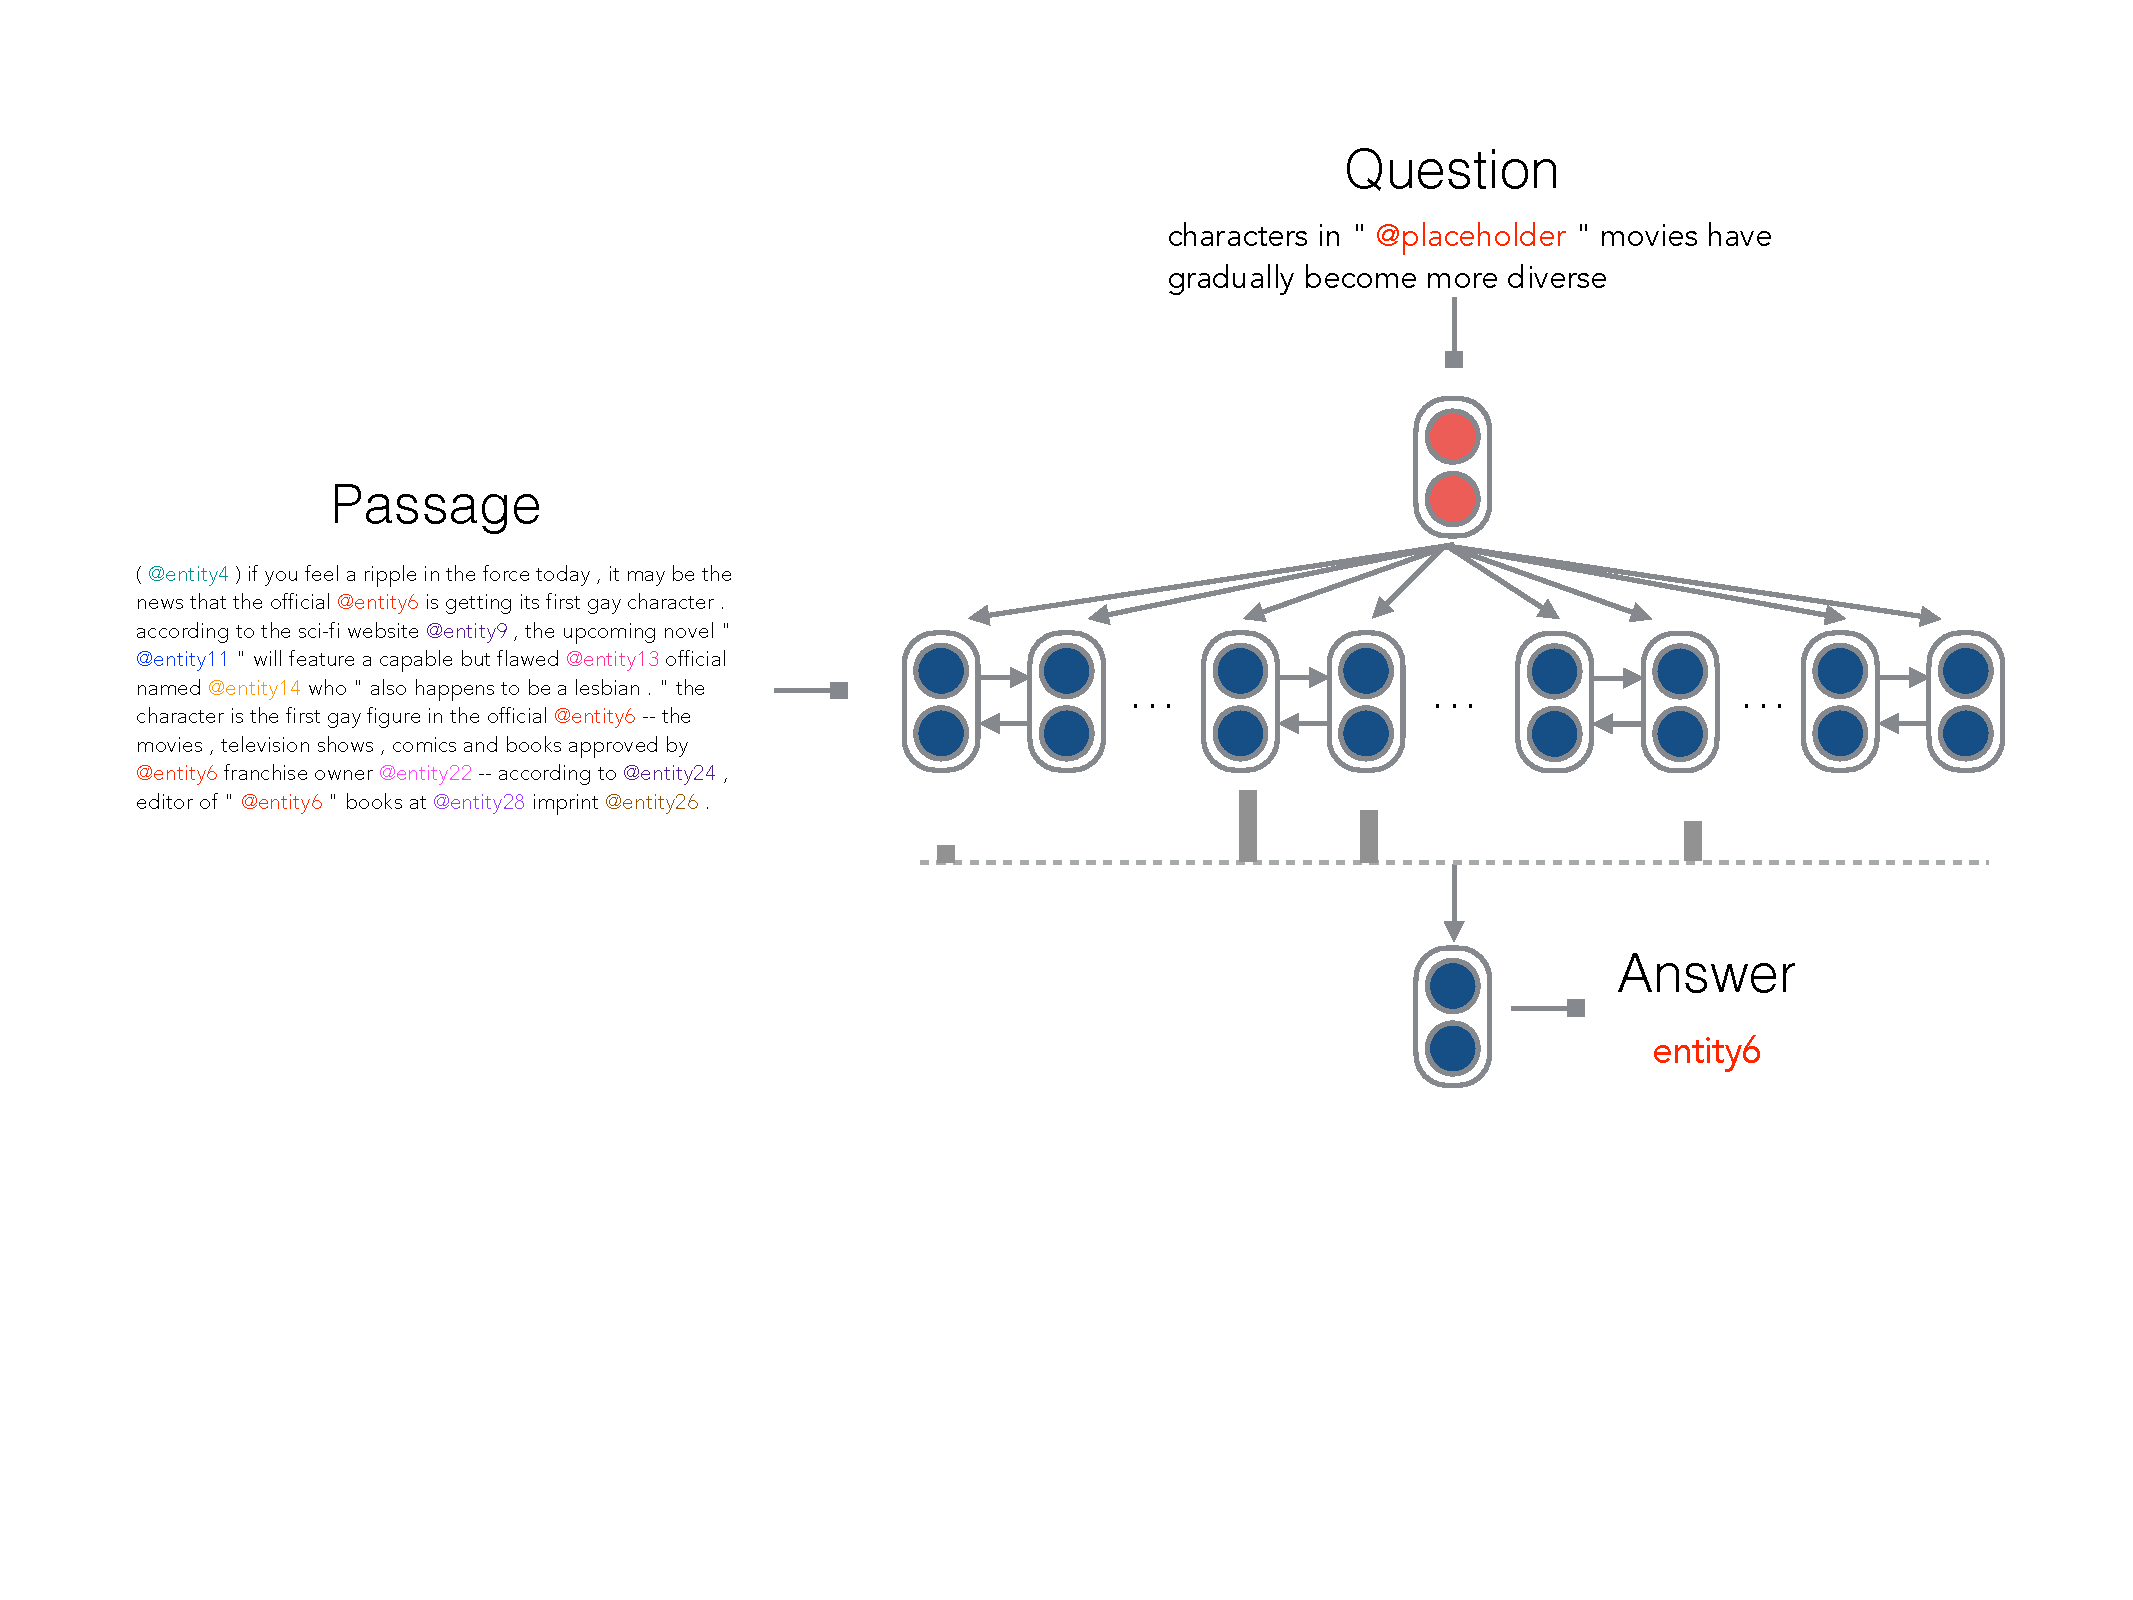
\includegraphics[scale=0.37]{figures/fig_model.pdf}
\caption{Our neural network architecture for the reading comprehension task.}
\label{fig:framework}
\end{figure*}

\begin{description}
    \item[\tf{Encoding:}] First, all the words are mapped to $d$-dimensional vectors via an embedding matrix $E \in \R^{d \times |\mathcal{V}|}$; therefore we have $p$: $\mf{p}_1, \ldots, \mf{p}_m \in R^d$ and $q: \mf{q}_1, \ldots, \mf{q}_{l} \in R^d$.

        Next we use a shallow bi-directional recurrent neural network (RNN) with hidden size $\tilde{h}$ to encode contextual embeddings $\tilde{\mf{p}}_i$ of each word in the passage,
        \begin{eqnarray*}
            \overrightarrow{\mf{h}}_i & = & \text{RNN}(\overrightarrow{\mf{h}}_{i-1}, \mf{p}_i), i = 1, \ldots, m\\
            \overleftarrow{\mf{h}}_i & = & \text{RNN}(\overleftarrow{\mf{h}}_{i+1}, \mf{p}_i), i = m, \ldots, 1
        \end{eqnarray*}
        and $\tilde{\mf{p}}_i = \text{concat}(\overrightarrow{\mf{h}}_i, \overleftarrow{\mf{h}}_i) \in \R^{h}$, where $h = 2 \tilde{h}$.
        Meanwhile, we use another bi-directional RNN to map the question $\mf{q}_1, \ldots, \mf{q}_l$ to an embedding $\mf{q} \in \R^h$. We choose to use Gated Recurrent Unit (GRU) \cite{cho2014learning} in our experiments because it performs similarly but is computationally cheaper than LSTM.

    \item[\tf{Attention:}] In this step, the goal is to compare the question embedding and all the contextual embeddings, and \ti{select} the pieces of information that are relevant to the question. We compute a probability distribution $\alpha$ depending on the degree of relevance between word $p_i$ (in its context) and the question $q$ and then produce an output vector $\mf{o}$ which is a weighted combination of all contextual embeddings $\{\tilde{\mf{p}}_i\}$:
        \begin{eqnarray}
            \alpha_i & = & \softmax\nolimits_i \mf{q} ^{\intercal} \mf{W}_{s} \tilde{\mf{p}}_i  \\
            \mf{o} & = & \sum\nolimits_{i}{\alpha_i \tilde{\mf{p}}_i}
        \end{eqnarray}
        $\mf{W_s} \in \R^{h \times h}$ is used in a bilinear term, which allows us to compute a similarity between $\mf{q}$ and $\tilde{\mf{p}}_i$ more flexibly than with just a dot product.
    \item[\tf{Prediction:}] Using the \ti{output} vector $\mf{o}$, the system outputs the most likely answer using:
        \begin{equation}
            a = \argmax\nolimits_{a \in p \cap E}{W_a ^{\intercal} \mf{o}}
        \end{equation}
        Finally, the system adds a softmax function on top of $W_a ^{\intercal} \mf{o}$ and adopts a negative log-likelihood objective for training.
\end{description}

\paragraph*{Differences from \cite{hermann2015teaching}.}
Our model basically follows the \ti{AttentiveReader}. However, to our surprise, our experiments observed nearly \tf{7} --\tf{10}\% improvement over the original \ti{AttentiveReader} results on \ti{CNN} and \ti{Daily Mail} datasets (discussed in Sec.~\ref{sec:experiments}). Concretely, our model has the following differences:
\begin{itemize}
\item
We use a bilinear term, instead of a $\tanh$ layer to compute the relevance (attention) between question and contextual embeddings. The effectiveness of the simple bilinear attention function has been shown previously for neural machine translation by \cite{luong2015effective}.
\item
After obtaining the weighted contextual embeddings $\mf{o}$, we use $\mf{o}$ for direct prediction. In contrast, the original model in \cite{hermann2015teaching} combined $\mf{o}$ and the question embedding $\mf{q}$ via another non-linear layer before making final predictions. We found that we could remove this layer without harming performance. We believe it is sufficient for the model to learn to return the entity to which it maximally gives attention.
\item
The original model considers all the words from the vocabulary $\mathcal{V}$ in making predictions. We think this is unnecessary, and only predict among entities which appear in the passage.
\end{itemize}
Of these changes, only the first seems important; the other two just aim at keeping the model simple.

\paragraph*{Window-based MemN2Ns \cite{hill2016goldilocks}.}
Another recent neural network approach proposed by \cite{hill2016goldilocks} is based on a memory network architecture \cite{weston2015memory}. We think it is highly similar in spirit. The biggest difference is their way of encoding passages: they demonstrate that it is most effective to only use a 5-word context window when evaluating a candidate entity and they use a positional unigram approach to encode the contextual embeddings: if a window consists of 5 words $x_1, \ldots, x_5$, then it is encoded as $\sum_{i=1}^{5}{E_i(x_i)}$, resulting in $5$ separate embedding matrices to learn. They encode the 5-word window surrounding the placeholder in a similar way and all other words in the question text are ignored. In addition, they simply use a dot product to compute the ``relevance'' between the question and a contextual embedding. This simple model nevertheless works well, showing the extent to which this RC task can be done by very local context matching.

\section{Experiments}
\label{sect:experiments}

% \begin{figure*}
%   \centering
%   \setlength{\tabcolsep}{0pt}
%   \setlength\figurewidth{0.05\textwidth}
%   \newcommand{\example}[1]{\raisebox{-.4\height}{\includegraphics[width=\figurewidth]{./figures/domains_examples/#1}}}
%   \begin{sc}
%   \begin{tabular}{r@{\hskip 1cm} ccccccccccc}
%     MNIST \cite{LeCun98} &
%     \example{mnist_0.png} &
%     \example{mnist_1.png} &
%     \example{mnist_2.png} &
%     \example{mnist_3.png} &
%     \example{mnist_4.png} &
%     \example{mnist_5.png} &
%     \example{mnist_6.png} &
%     \example{mnist_7.png} &
%     \example{mnist_8.png} &
%     \example{mnist_9.png} &
%     \example{mnist_10.png}\\
%     MNIST ($ | \Delta | $, BG) &
%     \example{mnisti_0.png} &
%     \example{mnisti_1.png} &
%     \example{mnisti_2.png} &
%     \example{mnisti_3.png} &
%     \example{mnisti_4.png} &
%     \example{mnisti_5.png} &
%     \example{mnisti_6.png} &
%     \example{mnisti_7.png} &
%     \example{mnisti_8.png} &
%     \example{mnisti_9.png} &
%     \example{mnisti_10.png}\\
%     Syn Numbers &
%     \example{syn_0.png} &
%     \example{syn_1.png} &
%     \example{syn_2.png} &
%     \example{syn_3.png} &
%     \example{syn_4.png} &
%     \example{syn_5.png} &
%     \example{syn_6.png} &
%     \example{syn_7.png} &
%     \example{syn_8.png} &
%     \example{syn_9.png} &
%     \example{syn_10.png}\\
%     SVHN \cite{Netzer11} &
%     \example{svhn_0.png} &
%     \example{svhn_1.png} &
%     \example{svhn_2.png} &
%     \example{svhn_3.png} &
%     \example{svhn_4.png} &
%     \example{svhn_5.png} &
%     \example{svhn_6.png} &
%     \example{svhn_7.png} &
%     \example{svhn_8.png} &
%     \example{svhn_9.png} &
%     \example{svhn_10.png}\\
%     Syn Signs &
%     \example{synsgn_11.png} &
%     \example{synsgn_1.png} &
%     \example{synsgn_2.png} &
%     \example{synsgn_3.png} &
%     \example{synsgn_4.png} &
%     \example{synsgn_5.png} &
%     \example{synsgn_12.png} &
%     \example{synsgn_7.png} &
%     \example{synsgn_8.png} &
%     \example{synsgn_9.png} &
%     \example{synsgn_10.png}\\
%     GTSRB \cite{Stallkamp12} &
%     \example{gtsrb_0.png} &
%     \example{gtsrb_1.png} &
%     \example{gtsrb_2.png} &
%     \example{gtsrb_3.png} &
%     \example{gtsrb_4.png} &
%     \example{gtsrb_5.png} &
%     \example{gtsrb_6.png} &
%     \example{gtsrb_7.png} &
%     \example{gtsrb_8.png} &
%     \example{gtsrb_9.png} &
%     \example{gtsrb_10.png}\\
%     % CIFAR-10 \cite{Krizhevsky09} &
%     % \example{cifar10_0.png} &
%     % \example{cifar10_1.png} &
%     % \example{cifar10_2.png} &
%     % \example{cifar10_3.png} &
%     % \example{cifar10_4.png} &
%     % \example{cifar10_5.png} &
%     % \example{cifar10_11.png} &
%     % \example{cifar10_7.png} &
%     % \example{cifar10_8.png} &
%     % \example{cifar10_9.png} &
%     % \example{cifar10_10.png}\\
%     % STL-10 \cite{Coates11} &
%     % \example{stl10_12.png} &
%     % \example{stl10_1.png} &
%     % \example{stl10_2.png} &
%     % \example{stl10_3.png} &
%     % \example{stl10_4.png} &
%     % \example{stl10_5.png} &
%     % \example{stl10_6.png} &
%     % \example{stl10_13.png} &
%     % \example{stl10_8.png} &
%     % \example{stl10_9.png} &
%     % \example{stl10_10.png}\\
%   \end{tabular}
%   \end{sc}
%   \vskip 2.5mm
%   \caption{\todo[What to do with this figure? Add Office? Remove?]Random samples from the datasets used in the experiments. See \sect{exper_quant} for details.}
%   \label{fig:exper_domains_examples}
% \end{figure*}

\begin{figure*}
  \centering
  \setlength{\tabcolsep}{0pt}
  \setlength\figurewidth{0.05\textwidth}
  \newcommand{\example}[1]{\raisebox{-.4\height}{\includegraphics[width=\figurewidth]{./figures/domains_examples/#1}}}
  \begin{sc}
  \begin{small}
  \begin{tabular}{r@{\hskip 0.5cm} ccc c@{\hskip 0.4cm} ccc c@{\hskip 0.4cm} ccc c@{\hskip 0.4cm} ccc}
    &
    \multicolumn{3}{c}{MNIST} & &
    \multicolumn{3}{c}{Syn Numbers} & &
    \multicolumn{3}{c}{SVHN} & &
    \multicolumn{3}{c}{Syn Signs}\\
    
    Source &
    \example{mnist_0.png} &
    \example{mnist_1.png} &
    \example{mnist_3.png} & &
    
    \example{syn_0.png} &
    \example{syn_1.png} &
    \example{syn_2.png} & &
    
    \example{svhn_3.png} &
    \example{svhn_4.png} &
    \example{svhn_5.png} & &
    
    \example{synsgn_3.png} &
    \example{synsgn_4.png} &
    \example{synsgn_5.png}\\
    
    Target &
    \example{mnisti_0.png} &
    \example{mnisti_1.png} &
    \example{mnisti_2.png} & &
    
    \example{svhn_0.png} &
    \example{svhn_1.png} &
    \example{svhn_2.png} & &
    
    \example{mnist_4.png} &
    \example{mnist_5.png} &
    \example{mnist_6.png} & &
    
    \example{gtsrb_2.png} &
    \example{gtsrb_3.png} &
    \example{gtsrb_4.png}\\
    
    &
    \multicolumn{3}{c}{\rule{0pt}{0.35cm} MNIST-M} & &
    \multicolumn{3}{c}{SVHN} & &
    \multicolumn{3}{c}{MNIST} & &
    \multicolumn{3}{c}{GTSRB}\\
  \end{tabular}
  \end{small}
  \end{sc}
  \caption{Examples of domain pairs used in the experiments. See \sect{exper_quant} for details.}
  \label{fig:exper_domains_examples}
\end{figure*}


\begin{table*}[t]
  \vskip 0.15in
  \begin{center}
    \begin{small}
      \begin{sc}
        \renewcommand{\arraystretch}{1.5}
        \begin{tabular}{l r | c c c c}
          \hline
          \multirow{2}{*}{Method} & {\scriptsize Source} & MNIST & Syn Numbers & SVHN & Syn Signs \\
          & {\scriptsize Target} & MNIST-M & SVHN & MNIST & GTSRB \\
          \hline
          \multicolumn{2}{l |}{Source only} & 
          $ .5749 $                      & $ .8665 $                      & $ .5919 $                      & $ .7400 $                      \\
          \multicolumn{2}{l |}{SA \cite{Fernando13}} & 
          $ .6078 \; (7.9\%) $           & $ .8672 \; (1.3\%) $           & $ .6157 \; (5.9\%) $           & $ .7635 \; (9.1\%) $           \\
          \multicolumn{2}{l |}{Proposed approach} & 
          $ \mathbf{.8149} \; (57.9\%) $ & $ \mathbf{.9048} \; (66.1\%) $ & $ \mathbf{.7107} \; (29.3\%) $ & $ \mathbf{.8866} \; (56.7\%) $ \\
          \multicolumn{2}{l |}{Train on target} & 
          $ .9891 $                      & $ .9244 $                      & $ .9951 $                      & $ .9987 $                      \\
          \hline
        \end{tabular}
      \end{sc}
    \end{small}
  \end{center}
    \caption{Classification accuracies for digit image classifications for different source and target domains. {\sc MNIST-M} corresponds to difference-blended digits over non-uniform background. The first row corresponds to the lower performance bound (i.e.\ if no adaptation is performed). The last row corresponds to training on the target domain data with known class labels (upper bound on the DA performance). For each of the two DA methods (ours and \cite{Fernando13}) we show how much of the gap between the lower and the upper bounds was covered (in brackets). For all five cases, our approach outperforms \cite{Fernando13} considerably, and covers a big portion of the gap.\vspace{-0mm} }
  \label{tab:results}
  \vskip -0.1in
\end{table*}

\begin{table*}[t]
  \vskip 0.15in
  \begin{center}
    \begin{small}
      \begin{sc}
        \renewcommand{\arraystretch}{1.5}
        \begin{tabular}{l r | c c c}
          \hline
          \multirow{2}{*}{Method} & {\scriptsize Source} & Amazon & DSLR & Webcam \\
          & {\scriptsize Target} & Webcam & Webcam & DSLR \\
          \hline
          \multicolumn{2}{l |}{GFK(PLS, PCA) \cite{Gong12}} & 
          $ .464 \pm .005 $ & $ .613 \pm .004 $ & $ .663 \pm .004 $\\ 
          \multicolumn{2}{l |}{SA \cite{Fernando13}} & 
          $ .450 $ & $ .648 $ & $ .699 $\\ 
          \multicolumn{2}{l |}{DA-NBNN \cite{Tommasi13}} & 
          $ .528 \pm .037 $ & $ .766 \pm .017 $ & $ .762 \pm .025 $\\ 
          \multicolumn{2}{l |}{DLID \cite{Chopra13}} & 
          $ .519 $ & $ .782 $ & $ .899 $\\
          \multicolumn{2}{l |}{DeCAF$_6$ Source Only \cite{Donahue14}} &
          $ .522 \pm .017 $ & $ .915 \pm .015 $ & --\\ 
          \multicolumn{2}{l |}{DaNN \cite{Ghifary14}} & 
          $ .536 \pm .002 $ & $ .712 \pm .000 $ & $ .835 \pm .000 $\\ 
          \multicolumn{2}{l |}{DDC \cite{Tzeng14}} & 
          $ .594 \pm .008 $ & $ .925 \pm .003 $ & $ .917 \pm .008 $\\ 
          \multicolumn{2}{l |}{Proposed Approach} & 
          $ \mathbf{ .673 \pm .017 } $ & $ \mathbf{ .940 \pm .008 } $ & $ \mathbf{ .937 \pm .010 } $\\
          \hline
        \end{tabular}
      \end{sc}
    \end{small}
  \end{center}
    \caption{Accuracy evaluation of different DA approaches on the standard {\sc Office} \cite{Saenko10} dataset. Our method (last row) outperforms competitors setting the new state-of-the-art.}
  \label{tab:results_office}
\end{table*}

% Other rows refer to the following algorithms (from top to bottom): Geodesic Flow Kernel \cite{Gong12}, Subspace Alignment \cite{Fernando13}, Naive Bayes Nearest Neighbor \cite{Tommasi13},  deep learning approach from \cite{Chopra13}, DeCAF$_6$-features described in \cite{Donahue14}, Domain Adaptive NNs \cite{Ghifary14}, Deep Domain Confusion \cite{Tzeng14}.

\def\X{{\mathbf X}}
\def\y{{\mathbf y}}

% \vspace{2mm}\noindent {\bf Datasets.}
% \label{sect:exper_datasets}

% In order to test our method in the setting of traffic signs classification we obtained~100,000 synthetic images ({\sc Syn~Signs}) simulating various photoshooting conditions. This dataset was used in conjunction with {\it The German Traffic Sign Recognition Benchmark} ({\sc GTSRB}) \cite{Stallkamp12}.

% Finally, we perform domain adaption for the {\sc CIFAR-10} and the {\sc STL-10} downsampled to the size of $ 32 \times 32 $. This pair is considerably different from the previously mentioned datasets as the intra-class variability here is higher.

We perform extensive evaluation of the proposed approach on a number of popular image datasets and their modifications. These include large-scale datasets of small images popular with deep learning methods, and the {\sc Office} datasets \cite{Saenko10}, which are a {\em de facto} standard for domain adaptation in computer vision, but have much fewer images.

\vspace{2mm}\noindent {\bf Baselines.} For the bulk of experiments the following baselines are evaluated. The \textbf{source-only} model is trained without consideration for target-domain data (no domain classifier branch included into the network). The \textbf{train-on-target} model is trained on the target domain with class labels revealed. This model serves as an upper bound on DA methods, assuming that target data are abundant and the shift between the domains is considerable. 

In addition, we compare our approach against the recently proposed unsupervised DA method based on \textbf{subspace alignment (SA)} \cite{Fernando13}, which is simple to setup and test on new datasets, but has also been shown to perform very well in experimental comparisons with other ``shallow'' DA methods. To boost the performance of this baseline, we pick its most important free parameter (the number of principal components) from the range $ \{ 2, \ldots, 60 \} $, so that the test performance on the target domain is maximized. To apply SA in our setting, we train a source-only model and then consider the activations of the last hidden layer in the label predictor (before the final linear classifier) as descriptors/features, and learn the mapping between the source and the target domains \cite{Fernando13}.

Since the SA baseline requires to train a new classifier after adapting the features, and in order to put all the compared settings on an equal footing, we retrain the last layer of the label predictor using a standard linear SVM~\cite{liblinear} for all four considered methods (including ours; the performance on the target domain remains approximately the same after the retraining). 

For the {\sc Office} dataset \cite{Saenko10}, we directly compare the performance of our full network (feature extractor and label predictor) against recent DA approaches using previously published results.

\vspace{2mm}\noindent {\bf CNN architectures.} In general, we compose feature extractor from two or three convolutional layers, picking their exact configurations from previous works. We give the exact architectures in \ref{sect:appendix_archs}.

For the domain adaptator we stick to the three fully connected layers ($x\rightarrow1024\rightarrow1024\rightarrow2$), except for {\sc MNIST} where we used a simpler ($x\rightarrow100\rightarrow2$) architecture to speed up the experiments.

For loss functions, we set $ L_y $ and $ L_d $ to be the logistic regression loss and the binomial cross-entropy respectively.

\vspace{2mm}\noindent {\bf CNN training procedure.}
The model is trained on $128$-sized batches. Images are preprocessed by the mean subtraction. A half of each batch is populated by the samples from the source domain (with known labels), the rest is comprised of the target domain (with unknown labels).

In order to suppress noisy signal from the domain classifier at the early stages of the training procedure instead of fixing the adaptation factor $ \lambda $, we gradually change it from $0$ to $1$ using the following schedule:
\begin{equation}
  \lambda_p = \frac{2}{1 + \exp(-\gamma \cdot p)} - 1,
\end{equation}
where $\gamma$ was set to $10$ in all experiments (the schedule was not optimized/tweaked). Further details on the CNN training can be found in \ref{sect:appendix_training}.

\vspace{2mm}\noindent {\bf Visualizations.}
We use t-SNE \cite{Maaten13} projection to visualize feature distributions at different points of the network, while color-coding the domains (\fig{exper_adapt_vis}). We observe strong correspondence between the success of the adaptation in terms of the classification accuracy for the target domain, and the overlap between the domain distributions in such visualizations.
 
\vspace{2mm}\noindent {\bf Choosing meta-parameters.} 
In general, good unsupervised DA methods should provide ways to set meta-parameters (such as $\lambda$, the learning rate, the momentum rate, the network architecture for our method) in an unsupervised way, i.e.\ without referring to labeled data in the target domain. %Here we would like to give few recommendations concerning this matter. First, as it was pointed out in \sect{theory} the domain classifier should not be significantly more complex than the label predictor. 
In our method, one can assess the performance of the whole system (and the effect of changing hyper-parameters) by observing the test error on the source domain {\em and} the domain classifier error. In general, we observed a good correspondence between the success of adaptation and these errors (adaptation is more successful when the source domain test error is low, while the domain classifier error is high).
In addition, the layer, where the the domain adaptator is attached can be picked by computing difference between means as suggested in \cite{Tzeng14}. 

% \begin{figure*}
%   \centering
%   {\sc MNIST $ \rightarrow $ MNIST ($ | \Delta | $, bg)}: top feature extractor layer
%   \setcounter{subfigure}{0}
%   \subfigure[Non-adapted]{%%
%     \scalebox{0.8}{%% Creator: Matplotlib, PGF backend
%%
%% To include the figure in your LaTeX document, write
%%   \input{<filename>.pgf}
%%
%% Make sure the required packages are loaded in your preamble
%%   \usepackage{pgf}
%%
%% Figures using additional raster images can only be included by \input if
%% they are in the same directory as the main LaTeX file. For loading figures
%% from other directories you can use the `import` package
%%   \usepackage{import}
%% and then include the figures with
%%   \import{<path to file>}{<filename>.pgf}
%%
%% Matplotlib used the following preamble
%%   \usepackage[utf8x]{inputenc}
%%   \usepackage[T1]{fontenc}
%%
\begingroup%
\makeatletter%
\begin{pgfpicture}%
\pgfpathrectangle{\pgfpointorigin}{\pgfqpoint{3.338520in}{2.040000in}}%
\pgfusepath{use as bounding box}%
\begin{pgfscope}%
\pgfsetbuttcap%
\pgfsetroundjoin%
\definecolor{currentfill}{rgb}{1.000000,1.000000,1.000000}%
\pgfsetfillcolor{currentfill}%
\pgfsetlinewidth{0.000000pt}%
\definecolor{currentstroke}{rgb}{1.000000,1.000000,1.000000}%
\pgfsetstrokecolor{currentstroke}%
\pgfsetdash{}{0pt}%
\pgfpathmoveto{\pgfqpoint{0.000000in}{-0.000000in}}%
\pgfpathlineto{\pgfqpoint{3.338520in}{-0.000000in}}%
\pgfpathlineto{\pgfqpoint{3.338520in}{2.040000in}}%
\pgfpathlineto{\pgfqpoint{0.000000in}{2.040000in}}%
\pgfpathclose%
\pgfusepath{fill}%
\end{pgfscope}%
\begin{pgfscope}%
\pgftext[at=\pgfqpoint{0.510000in}{0.348333in},left,bottom]{\pgfimage[interpolate=true,width=2.553333in,height=1.500000in]{./figures/adaptation_vis/pool2_mnist2inv_before-img0.png}}%
\end{pgfscope}%
\begin{pgfscope}%
\pgftext[at=\pgfqpoint{0.805000in}{0.383333in},left,bottom]{\pgfimage[interpolate=true,width=2.201667in,height=1.371667in]{./figures/adaptation_vis/pool2_mnist2inv_before-img1.png}}%
\end{pgfscope}%
\end{pgfpicture}%
\makeatother%
\endgroup%
}}%%
%   \subfigure[Adapted]{%%
%     \scalebox{0.8}{%% Creator: Matplotlib, PGF backend
%%
%% To include the figure in your LaTeX document, write
%%   \input{<filename>.pgf}
%%
%% Make sure the required packages are loaded in your preamble
%%   \usepackage{pgf}
%%
%% Figures using additional raster images can only be included by \input if
%% they are in the same directory as the main LaTeX file. For loading figures
%% from other directories you can use the `import` package
%%   \usepackage{import}
%% and then include the figures with
%%   \import{<path to file>}{<filename>.pgf}
%%
%% Matplotlib used the following preamble
%%   \usepackage[utf8x]{inputenc}
%%   \usepackage[T1]{fontenc}
%%
\begingroup%
\makeatletter%
\begin{pgfpicture}%
\pgfpathrectangle{\pgfpointorigin}{\pgfqpoint{3.340000in}{2.040000in}}%
\pgfusepath{use as bounding box}%
\begin{pgfscope}%
\pgfsetbuttcap%
\pgfsetroundjoin%
\definecolor{currentfill}{rgb}{1.000000,1.000000,1.000000}%
\pgfsetfillcolor{currentfill}%
\pgfsetlinewidth{0.000000pt}%
\definecolor{currentstroke}{rgb}{1.000000,1.000000,1.000000}%
\pgfsetstrokecolor{currentstroke}%
\pgfsetdash{}{0pt}%
\pgfpathmoveto{\pgfqpoint{0.000000in}{-0.000000in}}%
\pgfpathlineto{\pgfqpoint{3.340000in}{-0.000000in}}%
\pgfpathlineto{\pgfqpoint{3.340000in}{2.040000in}}%
\pgfpathlineto{\pgfqpoint{0.000000in}{2.040000in}}%
\pgfpathclose%
\pgfusepath{fill}%
\end{pgfscope}%
\begin{pgfscope}%
\pgftext[at=\pgfqpoint{0.518333in}{0.321667in},left,bottom]{\pgfimage[interpolate=true,width=2.565000in,height=1.550000in]{./figures/adaptation_vis/pool2_mnist2inv_after-img0.png}}%
\end{pgfscope}%
\begin{pgfscope}%
\pgftext[at=\pgfqpoint{0.518333in}{0.321667in},left,bottom]{\pgfimage[interpolate=true,width=2.565000in,height=1.553333in]{./figures/adaptation_vis/pool2_mnist2inv_after-img1.png}}%
\end{pgfscope}%
\end{pgfpicture}%
\makeatother%
\endgroup%
}}\\
%   \vspace{5mm}
%   {\sc Syn Numbers $ \rightarrow $ SVHN}: last hidden layer of the label predictor
%   \setcounter{subfigure}{0}
%   \subfigure[Non-adapted]{%%
%     \scalebox{0.8}{%% Creator: Matplotlib, PGF backend
%%
%% To include the figure in your LaTeX document, write
%%   \input{<filename>.pgf}
%%
%% Make sure the required packages are loaded in your preamble
%%   \usepackage{pgf}
%%
%% Figures using additional raster images can only be included by \input if
%% they are in the same directory as the main LaTeX file. For loading figures
%% from other directories you can use the `import` package
%%   \usepackage{import}
%% and then include the figures with
%%   \import{<path to file>}{<filename>.pgf}
%%
%% Matplotlib used the following preamble
%%   \usepackage[utf8x]{inputenc}
%%   \usepackage[T1]{fontenc}
%%
\begingroup%
\makeatletter%
\begin{pgfpicture}%
\pgfpathrectangle{\pgfpointorigin}{\pgfqpoint{3.340000in}{2.040000in}}%
\pgfusepath{use as bounding box}%
\begin{pgfscope}%
\pgfsetbuttcap%
\pgfsetroundjoin%
\definecolor{currentfill}{rgb}{1.000000,1.000000,1.000000}%
\pgfsetfillcolor{currentfill}%
\pgfsetlinewidth{0.000000pt}%
\definecolor{currentstroke}{rgb}{1.000000,1.000000,1.000000}%
\pgfsetstrokecolor{currentstroke}%
\pgfsetdash{}{0pt}%
\pgfpathmoveto{\pgfqpoint{0.000000in}{-0.000000in}}%
\pgfpathlineto{\pgfqpoint{3.340000in}{-0.000000in}}%
\pgfpathlineto{\pgfqpoint{3.340000in}{2.040000in}}%
\pgfpathlineto{\pgfqpoint{0.000000in}{2.040000in}}%
\pgfpathclose%
\pgfusepath{fill}%
\end{pgfscope}%
\begin{pgfscope}%
\pgftext[at=\pgfqpoint{0.491667in}{0.335000in},left,bottom]{\pgfimage[interpolate=true,width=2.618333in,height=1.531667in]{./figures/adaptation_vis/before-img0.png}}%
\end{pgfscope}%
\begin{pgfscope}%
\pgftext[at=\pgfqpoint{0.758333in}{0.331667in},left,bottom]{\pgfimage[interpolate=true,width=2.171667in,height=1.436667in]{./figures/adaptation_vis/before-img1.png}}%
\end{pgfscope}%
\begin{pgfscope}%
\pgfsetbuttcap%
\pgfsetroundjoin%
\definecolor{currentfill}{rgb}{0.000000,0.000000,1.000000}%
\pgfsetfillcolor{currentfill}%
\pgfsetfillopacity{0.300000}%
\pgfsetlinewidth{0.150562pt}%
\definecolor{currentstroke}{rgb}{0.000000,0.000000,0.000000}%
\pgfsetstrokecolor{currentstroke}%
\pgfsetstrokeopacity{0.300000}%
\pgfsetdash{}{0pt}%
\pgfpathmoveto{\pgfqpoint{2.521160in}{1.775861in}}%
\pgfpathcurveto{\pgfqpoint{2.525278in}{1.775861in}}{\pgfqpoint{2.529228in}{1.777497in}}{\pgfqpoint{2.532140in}{1.780409in}}%
\pgfpathcurveto{\pgfqpoint{2.535052in}{1.783321in}}{\pgfqpoint{2.536688in}{1.787271in}}{\pgfqpoint{2.536688in}{1.791389in}}%
\pgfpathcurveto{\pgfqpoint{2.536688in}{1.795507in}}{\pgfqpoint{2.535052in}{1.799457in}}{\pgfqpoint{2.532140in}{1.802369in}}%
\pgfpathcurveto{\pgfqpoint{2.529228in}{1.805281in}}{\pgfqpoint{2.525278in}{1.806917in}}{\pgfqpoint{2.521160in}{1.806917in}}%
\pgfpathcurveto{\pgfqpoint{2.517042in}{1.806917in}}{\pgfqpoint{2.513092in}{1.805281in}}{\pgfqpoint{2.510180in}{1.802369in}}%
\pgfpathcurveto{\pgfqpoint{2.507268in}{1.799457in}}{\pgfqpoint{2.505631in}{1.795507in}}{\pgfqpoint{2.505631in}{1.791389in}}%
\pgfpathcurveto{\pgfqpoint{2.505631in}{1.787271in}}{\pgfqpoint{2.507268in}{1.783321in}}{\pgfqpoint{2.510180in}{1.780409in}}%
\pgfpathcurveto{\pgfqpoint{2.513092in}{1.777497in}}{\pgfqpoint{2.517042in}{1.775861in}}{\pgfqpoint{2.521160in}{1.775861in}}%
\pgfpathclose%
\pgfusepath{stroke,fill}%
\end{pgfscope}%
\begin{pgfscope}%
\pgfsetbuttcap%
\pgfsetroundjoin%
\definecolor{currentfill}{rgb}{0.000000,0.000000,1.000000}%
\pgfsetfillcolor{currentfill}%
\pgfsetfillopacity{0.300000}%
\pgfsetlinewidth{0.150562pt}%
\definecolor{currentstroke}{rgb}{0.000000,0.000000,0.000000}%
\pgfsetstrokecolor{currentstroke}%
\pgfsetstrokeopacity{0.300000}%
\pgfsetdash{}{0pt}%
\pgfpathmoveto{\pgfqpoint{2.598938in}{1.785583in}}%
\pgfpathcurveto{\pgfqpoint{2.603056in}{1.785583in}}{\pgfqpoint{2.607006in}{1.787219in}}{\pgfqpoint{2.609918in}{1.790131in}}%
\pgfpathcurveto{\pgfqpoint{2.612830in}{1.793043in}}{\pgfqpoint{2.614466in}{1.796993in}}{\pgfqpoint{2.614466in}{1.801111in}}%
\pgfpathcurveto{\pgfqpoint{2.614466in}{1.805229in}}{\pgfqpoint{2.612830in}{1.809179in}}{\pgfqpoint{2.609918in}{1.812091in}}%
\pgfpathcurveto{\pgfqpoint{2.607006in}{1.815003in}}{\pgfqpoint{2.603056in}{1.816639in}}{\pgfqpoint{2.598938in}{1.816639in}}%
\pgfpathcurveto{\pgfqpoint{2.594819in}{1.816639in}}{\pgfqpoint{2.590869in}{1.815003in}}{\pgfqpoint{2.587957in}{1.812091in}}%
\pgfpathcurveto{\pgfqpoint{2.585045in}{1.809179in}}{\pgfqpoint{2.583409in}{1.805229in}}{\pgfqpoint{2.583409in}{1.801111in}}%
\pgfpathcurveto{\pgfqpoint{2.583409in}{1.796993in}}{\pgfqpoint{2.585045in}{1.793043in}}{\pgfqpoint{2.587957in}{1.790131in}}%
\pgfpathcurveto{\pgfqpoint{2.590869in}{1.787219in}}{\pgfqpoint{2.594819in}{1.785583in}}{\pgfqpoint{2.598938in}{1.785583in}}%
\pgfpathclose%
\pgfusepath{stroke,fill}%
\end{pgfscope}%
\begin{pgfscope}%
\pgfsetbuttcap%
\pgfsetroundjoin%
\definecolor{currentfill}{rgb}{0.000000,0.000000,1.000000}%
\pgfsetfillcolor{currentfill}%
\pgfsetfillopacity{0.300000}%
\pgfsetlinewidth{0.150562pt}%
\definecolor{currentstroke}{rgb}{0.000000,0.000000,0.000000}%
\pgfsetstrokecolor{currentstroke}%
\pgfsetstrokeopacity{0.300000}%
\pgfsetdash{}{0pt}%
\pgfpathmoveto{\pgfqpoint{2.676715in}{1.771000in}}%
\pgfpathcurveto{\pgfqpoint{2.680833in}{1.771000in}}{\pgfqpoint{2.684783in}{1.772636in}}{\pgfqpoint{2.687695in}{1.775548in}}%
\pgfpathcurveto{\pgfqpoint{2.690607in}{1.778460in}}{\pgfqpoint{2.692244in}{1.782410in}}{\pgfqpoint{2.692244in}{1.786528in}}%
\pgfpathcurveto{\pgfqpoint{2.692244in}{1.790646in}}{\pgfqpoint{2.690607in}{1.794596in}}{\pgfqpoint{2.687695in}{1.797508in}}%
\pgfpathcurveto{\pgfqpoint{2.684783in}{1.800420in}}{\pgfqpoint{2.680833in}{1.802056in}}{\pgfqpoint{2.676715in}{1.802056in}}%
\pgfpathcurveto{\pgfqpoint{2.672597in}{1.802056in}}{\pgfqpoint{2.668647in}{1.800420in}}{\pgfqpoint{2.665735in}{1.797508in}}%
\pgfpathcurveto{\pgfqpoint{2.662823in}{1.794596in}}{\pgfqpoint{2.661187in}{1.790646in}}{\pgfqpoint{2.661187in}{1.786528in}}%
\pgfpathcurveto{\pgfqpoint{2.661187in}{1.782410in}}{\pgfqpoint{2.662823in}{1.778460in}}{\pgfqpoint{2.665735in}{1.775548in}}%
\pgfpathcurveto{\pgfqpoint{2.668647in}{1.772636in}}{\pgfqpoint{2.672597in}{1.771000in}}{\pgfqpoint{2.676715in}{1.771000in}}%
\pgfpathclose%
\pgfusepath{stroke,fill}%
\end{pgfscope}%
\begin{pgfscope}%
\pgftext[x=2.798938in,y=1.762222in,left,base]{{\rmfamily\fontsize{8.000000}{9.600000}\selectfont Source}}%
\end{pgfscope}%
\begin{pgfscope}%
\pgfsetbuttcap%
\pgfsetroundjoin%
\definecolor{currentfill}{rgb}{1.000000,0.000000,0.000000}%
\pgfsetfillcolor{currentfill}%
\pgfsetfillopacity{0.300000}%
\pgfsetlinewidth{0.150562pt}%
\definecolor{currentstroke}{rgb}{0.000000,0.000000,0.000000}%
\pgfsetstrokecolor{currentstroke}%
\pgfsetstrokeopacity{0.300000}%
\pgfsetdash{}{0pt}%
\pgfpathmoveto{\pgfqpoint{2.521160in}{1.620928in}}%
\pgfpathcurveto{\pgfqpoint{2.525278in}{1.620928in}}{\pgfqpoint{2.529228in}{1.622564in}}{\pgfqpoint{2.532140in}{1.625476in}}%
\pgfpathcurveto{\pgfqpoint{2.535052in}{1.628388in}}{\pgfqpoint{2.536688in}{1.632338in}}{\pgfqpoint{2.536688in}{1.636456in}}%
\pgfpathcurveto{\pgfqpoint{2.536688in}{1.640574in}}{\pgfqpoint{2.535052in}{1.644524in}}{\pgfqpoint{2.532140in}{1.647436in}}%
\pgfpathcurveto{\pgfqpoint{2.529228in}{1.650348in}}{\pgfqpoint{2.525278in}{1.651984in}}{\pgfqpoint{2.521160in}{1.651984in}}%
\pgfpathcurveto{\pgfqpoint{2.517042in}{1.651984in}}{\pgfqpoint{2.513092in}{1.650348in}}{\pgfqpoint{2.510180in}{1.647436in}}%
\pgfpathcurveto{\pgfqpoint{2.507268in}{1.644524in}}{\pgfqpoint{2.505631in}{1.640574in}}{\pgfqpoint{2.505631in}{1.636456in}}%
\pgfpathcurveto{\pgfqpoint{2.505631in}{1.632338in}}{\pgfqpoint{2.507268in}{1.628388in}}{\pgfqpoint{2.510180in}{1.625476in}}%
\pgfpathcurveto{\pgfqpoint{2.513092in}{1.622564in}}{\pgfqpoint{2.517042in}{1.620928in}}{\pgfqpoint{2.521160in}{1.620928in}}%
\pgfpathclose%
\pgfusepath{stroke,fill}%
\end{pgfscope}%
\begin{pgfscope}%
\pgfsetbuttcap%
\pgfsetroundjoin%
\definecolor{currentfill}{rgb}{1.000000,0.000000,0.000000}%
\pgfsetfillcolor{currentfill}%
\pgfsetfillopacity{0.300000}%
\pgfsetlinewidth{0.150562pt}%
\definecolor{currentstroke}{rgb}{0.000000,0.000000,0.000000}%
\pgfsetstrokecolor{currentstroke}%
\pgfsetstrokeopacity{0.300000}%
\pgfsetdash{}{0pt}%
\pgfpathmoveto{\pgfqpoint{2.598938in}{1.630650in}}%
\pgfpathcurveto{\pgfqpoint{2.603056in}{1.630650in}}{\pgfqpoint{2.607006in}{1.632286in}}{\pgfqpoint{2.609918in}{1.635198in}}%
\pgfpathcurveto{\pgfqpoint{2.612830in}{1.638110in}}{\pgfqpoint{2.614466in}{1.642060in}}{\pgfqpoint{2.614466in}{1.646178in}}%
\pgfpathcurveto{\pgfqpoint{2.614466in}{1.650296in}}{\pgfqpoint{2.612830in}{1.654246in}}{\pgfqpoint{2.609918in}{1.657158in}}%
\pgfpathcurveto{\pgfqpoint{2.607006in}{1.660070in}}{\pgfqpoint{2.603056in}{1.661706in}}{\pgfqpoint{2.598938in}{1.661706in}}%
\pgfpathcurveto{\pgfqpoint{2.594819in}{1.661706in}}{\pgfqpoint{2.590869in}{1.660070in}}{\pgfqpoint{2.587957in}{1.657158in}}%
\pgfpathcurveto{\pgfqpoint{2.585045in}{1.654246in}}{\pgfqpoint{2.583409in}{1.650296in}}{\pgfqpoint{2.583409in}{1.646178in}}%
\pgfpathcurveto{\pgfqpoint{2.583409in}{1.642060in}}{\pgfqpoint{2.585045in}{1.638110in}}{\pgfqpoint{2.587957in}{1.635198in}}%
\pgfpathcurveto{\pgfqpoint{2.590869in}{1.632286in}}{\pgfqpoint{2.594819in}{1.630650in}}{\pgfqpoint{2.598938in}{1.630650in}}%
\pgfpathclose%
\pgfusepath{stroke,fill}%
\end{pgfscope}%
\begin{pgfscope}%
\pgfsetbuttcap%
\pgfsetroundjoin%
\definecolor{currentfill}{rgb}{1.000000,0.000000,0.000000}%
\pgfsetfillcolor{currentfill}%
\pgfsetfillopacity{0.300000}%
\pgfsetlinewidth{0.150562pt}%
\definecolor{currentstroke}{rgb}{0.000000,0.000000,0.000000}%
\pgfsetstrokecolor{currentstroke}%
\pgfsetstrokeopacity{0.300000}%
\pgfsetdash{}{0pt}%
\pgfpathmoveto{\pgfqpoint{2.676715in}{1.616066in}}%
\pgfpathcurveto{\pgfqpoint{2.680833in}{1.616066in}}{\pgfqpoint{2.684783in}{1.617703in}}{\pgfqpoint{2.687695in}{1.620615in}}%
\pgfpathcurveto{\pgfqpoint{2.690607in}{1.623527in}}{\pgfqpoint{2.692244in}{1.627477in}}{\pgfqpoint{2.692244in}{1.631595in}}%
\pgfpathcurveto{\pgfqpoint{2.692244in}{1.635713in}}{\pgfqpoint{2.690607in}{1.639663in}}{\pgfqpoint{2.687695in}{1.642575in}}%
\pgfpathcurveto{\pgfqpoint{2.684783in}{1.645487in}}{\pgfqpoint{2.680833in}{1.647123in}}{\pgfqpoint{2.676715in}{1.647123in}}%
\pgfpathcurveto{\pgfqpoint{2.672597in}{1.647123in}}{\pgfqpoint{2.668647in}{1.645487in}}{\pgfqpoint{2.665735in}{1.642575in}}%
\pgfpathcurveto{\pgfqpoint{2.662823in}{1.639663in}}{\pgfqpoint{2.661187in}{1.635713in}}{\pgfqpoint{2.661187in}{1.631595in}}%
\pgfpathcurveto{\pgfqpoint{2.661187in}{1.627477in}}{\pgfqpoint{2.662823in}{1.623527in}}{\pgfqpoint{2.665735in}{1.620615in}}%
\pgfpathcurveto{\pgfqpoint{2.668647in}{1.617703in}}{\pgfqpoint{2.672597in}{1.616066in}}{\pgfqpoint{2.676715in}{1.616066in}}%
\pgfpathclose%
\pgfusepath{stroke,fill}%
\end{pgfscope}%
\begin{pgfscope}%
\pgftext[x=2.798938in,y=1.607289in,left,base]{{\rmfamily\fontsize{8.000000}{9.600000}\selectfont Target}}%
\end{pgfscope}%
\end{pgfpicture}%
\makeatother%
\endgroup%
}}%%
%   \subfigure[Adapted]{%%
%     \scalebox{0.8}{%% Creator: Matplotlib, PGF backend
%%
%% To include the figure in your LaTeX document, write
%%   \input{<filename>.pgf}
%%
%% Make sure the required packages are loaded in your preamble
%%   \usepackage{pgf}
%%
%% Figures using additional raster images can only be included by \input if
%% they are in the same directory as the main LaTeX file. For loading figures
%% from other directories you can use the `import` package
%%   \usepackage{import}
%% and then include the figures with
%%   \import{<path to file>}{<filename>.pgf}
%%
%% Matplotlib used the following preamble
%%   \usepackage[utf8x]{inputenc}
%%   \usepackage[T1]{fontenc}
%%
\begingroup%
\makeatletter%
\begin{pgfpicture}%
\pgfpathrectangle{\pgfpointorigin}{\pgfqpoint{3.340000in}{2.040000in}}%
\pgfusepath{use as bounding box}%
\begin{pgfscope}%
\pgfsetbuttcap%
\pgfsetroundjoin%
\definecolor{currentfill}{rgb}{1.000000,1.000000,1.000000}%
\pgfsetfillcolor{currentfill}%
\pgfsetlinewidth{0.000000pt}%
\definecolor{currentstroke}{rgb}{1.000000,1.000000,1.000000}%
\pgfsetstrokecolor{currentstroke}%
\pgfsetdash{}{0pt}%
\pgfpathmoveto{\pgfqpoint{0.000000in}{-0.000000in}}%
\pgfpathlineto{\pgfqpoint{3.340000in}{-0.000000in}}%
\pgfpathlineto{\pgfqpoint{3.340000in}{2.040000in}}%
\pgfpathlineto{\pgfqpoint{0.000000in}{2.040000in}}%
\pgfpathclose%
\pgfusepath{fill}%
\end{pgfscope}%
\begin{pgfscope}%
\pgftext[at=\pgfqpoint{0.501667in}{0.330000in},left,bottom]{\pgfimage[interpolate=true,width=2.600000in,height=1.540000in]{./figures/adaptation_vis/after-img0.png}}%
\end{pgfscope}%
\begin{pgfscope}%
\pgftext[at=\pgfqpoint{0.500000in}{0.320000in},left,bottom]{\pgfimage[interpolate=true,width=2.585000in,height=1.556667in]{./figures/adaptation_vis/after-img1.png}}%
\end{pgfscope}%
\begin{pgfscope}%
\pgfsetbuttcap%
\pgfsetroundjoin%
\definecolor{currentfill}{rgb}{0.000000,0.000000,1.000000}%
\pgfsetfillcolor{currentfill}%
\pgfsetfillopacity{0.300000}%
\pgfsetlinewidth{0.150562pt}%
\definecolor{currentstroke}{rgb}{0.000000,0.000000,0.000000}%
\pgfsetstrokecolor{currentstroke}%
\pgfsetstrokeopacity{0.300000}%
\pgfsetdash{}{0pt}%
\pgfpathmoveto{\pgfqpoint{2.521160in}{1.775861in}}%
\pgfpathcurveto{\pgfqpoint{2.525278in}{1.775861in}}{\pgfqpoint{2.529228in}{1.777497in}}{\pgfqpoint{2.532140in}{1.780409in}}%
\pgfpathcurveto{\pgfqpoint{2.535052in}{1.783321in}}{\pgfqpoint{2.536688in}{1.787271in}}{\pgfqpoint{2.536688in}{1.791389in}}%
\pgfpathcurveto{\pgfqpoint{2.536688in}{1.795507in}}{\pgfqpoint{2.535052in}{1.799457in}}{\pgfqpoint{2.532140in}{1.802369in}}%
\pgfpathcurveto{\pgfqpoint{2.529228in}{1.805281in}}{\pgfqpoint{2.525278in}{1.806917in}}{\pgfqpoint{2.521160in}{1.806917in}}%
\pgfpathcurveto{\pgfqpoint{2.517042in}{1.806917in}}{\pgfqpoint{2.513092in}{1.805281in}}{\pgfqpoint{2.510180in}{1.802369in}}%
\pgfpathcurveto{\pgfqpoint{2.507268in}{1.799457in}}{\pgfqpoint{2.505631in}{1.795507in}}{\pgfqpoint{2.505631in}{1.791389in}}%
\pgfpathcurveto{\pgfqpoint{2.505631in}{1.787271in}}{\pgfqpoint{2.507268in}{1.783321in}}{\pgfqpoint{2.510180in}{1.780409in}}%
\pgfpathcurveto{\pgfqpoint{2.513092in}{1.777497in}}{\pgfqpoint{2.517042in}{1.775861in}}{\pgfqpoint{2.521160in}{1.775861in}}%
\pgfpathclose%
\pgfusepath{stroke,fill}%
\end{pgfscope}%
\begin{pgfscope}%
\pgfsetbuttcap%
\pgfsetroundjoin%
\definecolor{currentfill}{rgb}{0.000000,0.000000,1.000000}%
\pgfsetfillcolor{currentfill}%
\pgfsetfillopacity{0.300000}%
\pgfsetlinewidth{0.150562pt}%
\definecolor{currentstroke}{rgb}{0.000000,0.000000,0.000000}%
\pgfsetstrokecolor{currentstroke}%
\pgfsetstrokeopacity{0.300000}%
\pgfsetdash{}{0pt}%
\pgfpathmoveto{\pgfqpoint{2.598938in}{1.785583in}}%
\pgfpathcurveto{\pgfqpoint{2.603056in}{1.785583in}}{\pgfqpoint{2.607006in}{1.787219in}}{\pgfqpoint{2.609918in}{1.790131in}}%
\pgfpathcurveto{\pgfqpoint{2.612830in}{1.793043in}}{\pgfqpoint{2.614466in}{1.796993in}}{\pgfqpoint{2.614466in}{1.801111in}}%
\pgfpathcurveto{\pgfqpoint{2.614466in}{1.805229in}}{\pgfqpoint{2.612830in}{1.809179in}}{\pgfqpoint{2.609918in}{1.812091in}}%
\pgfpathcurveto{\pgfqpoint{2.607006in}{1.815003in}}{\pgfqpoint{2.603056in}{1.816639in}}{\pgfqpoint{2.598938in}{1.816639in}}%
\pgfpathcurveto{\pgfqpoint{2.594819in}{1.816639in}}{\pgfqpoint{2.590869in}{1.815003in}}{\pgfqpoint{2.587957in}{1.812091in}}%
\pgfpathcurveto{\pgfqpoint{2.585045in}{1.809179in}}{\pgfqpoint{2.583409in}{1.805229in}}{\pgfqpoint{2.583409in}{1.801111in}}%
\pgfpathcurveto{\pgfqpoint{2.583409in}{1.796993in}}{\pgfqpoint{2.585045in}{1.793043in}}{\pgfqpoint{2.587957in}{1.790131in}}%
\pgfpathcurveto{\pgfqpoint{2.590869in}{1.787219in}}{\pgfqpoint{2.594819in}{1.785583in}}{\pgfqpoint{2.598938in}{1.785583in}}%
\pgfpathclose%
\pgfusepath{stroke,fill}%
\end{pgfscope}%
\begin{pgfscope}%
\pgfsetbuttcap%
\pgfsetroundjoin%
\definecolor{currentfill}{rgb}{0.000000,0.000000,1.000000}%
\pgfsetfillcolor{currentfill}%
\pgfsetfillopacity{0.300000}%
\pgfsetlinewidth{0.150562pt}%
\definecolor{currentstroke}{rgb}{0.000000,0.000000,0.000000}%
\pgfsetstrokecolor{currentstroke}%
\pgfsetstrokeopacity{0.300000}%
\pgfsetdash{}{0pt}%
\pgfpathmoveto{\pgfqpoint{2.676715in}{1.771000in}}%
\pgfpathcurveto{\pgfqpoint{2.680833in}{1.771000in}}{\pgfqpoint{2.684783in}{1.772636in}}{\pgfqpoint{2.687695in}{1.775548in}}%
\pgfpathcurveto{\pgfqpoint{2.690607in}{1.778460in}}{\pgfqpoint{2.692244in}{1.782410in}}{\pgfqpoint{2.692244in}{1.786528in}}%
\pgfpathcurveto{\pgfqpoint{2.692244in}{1.790646in}}{\pgfqpoint{2.690607in}{1.794596in}}{\pgfqpoint{2.687695in}{1.797508in}}%
\pgfpathcurveto{\pgfqpoint{2.684783in}{1.800420in}}{\pgfqpoint{2.680833in}{1.802056in}}{\pgfqpoint{2.676715in}{1.802056in}}%
\pgfpathcurveto{\pgfqpoint{2.672597in}{1.802056in}}{\pgfqpoint{2.668647in}{1.800420in}}{\pgfqpoint{2.665735in}{1.797508in}}%
\pgfpathcurveto{\pgfqpoint{2.662823in}{1.794596in}}{\pgfqpoint{2.661187in}{1.790646in}}{\pgfqpoint{2.661187in}{1.786528in}}%
\pgfpathcurveto{\pgfqpoint{2.661187in}{1.782410in}}{\pgfqpoint{2.662823in}{1.778460in}}{\pgfqpoint{2.665735in}{1.775548in}}%
\pgfpathcurveto{\pgfqpoint{2.668647in}{1.772636in}}{\pgfqpoint{2.672597in}{1.771000in}}{\pgfqpoint{2.676715in}{1.771000in}}%
\pgfpathclose%
\pgfusepath{stroke,fill}%
\end{pgfscope}%
\begin{pgfscope}%
\pgftext[x=2.798938in,y=1.762222in,left,base]{{\rmfamily\fontsize{8.000000}{9.600000}\selectfont Source}}%
\end{pgfscope}%
\begin{pgfscope}%
\pgfsetbuttcap%
\pgfsetroundjoin%
\definecolor{currentfill}{rgb}{1.000000,0.000000,0.000000}%
\pgfsetfillcolor{currentfill}%
\pgfsetfillopacity{0.300000}%
\pgfsetlinewidth{0.150562pt}%
\definecolor{currentstroke}{rgb}{0.000000,0.000000,0.000000}%
\pgfsetstrokecolor{currentstroke}%
\pgfsetstrokeopacity{0.300000}%
\pgfsetdash{}{0pt}%
\pgfpathmoveto{\pgfqpoint{2.521160in}{1.620928in}}%
\pgfpathcurveto{\pgfqpoint{2.525278in}{1.620928in}}{\pgfqpoint{2.529228in}{1.622564in}}{\pgfqpoint{2.532140in}{1.625476in}}%
\pgfpathcurveto{\pgfqpoint{2.535052in}{1.628388in}}{\pgfqpoint{2.536688in}{1.632338in}}{\pgfqpoint{2.536688in}{1.636456in}}%
\pgfpathcurveto{\pgfqpoint{2.536688in}{1.640574in}}{\pgfqpoint{2.535052in}{1.644524in}}{\pgfqpoint{2.532140in}{1.647436in}}%
\pgfpathcurveto{\pgfqpoint{2.529228in}{1.650348in}}{\pgfqpoint{2.525278in}{1.651984in}}{\pgfqpoint{2.521160in}{1.651984in}}%
\pgfpathcurveto{\pgfqpoint{2.517042in}{1.651984in}}{\pgfqpoint{2.513092in}{1.650348in}}{\pgfqpoint{2.510180in}{1.647436in}}%
\pgfpathcurveto{\pgfqpoint{2.507268in}{1.644524in}}{\pgfqpoint{2.505631in}{1.640574in}}{\pgfqpoint{2.505631in}{1.636456in}}%
\pgfpathcurveto{\pgfqpoint{2.505631in}{1.632338in}}{\pgfqpoint{2.507268in}{1.628388in}}{\pgfqpoint{2.510180in}{1.625476in}}%
\pgfpathcurveto{\pgfqpoint{2.513092in}{1.622564in}}{\pgfqpoint{2.517042in}{1.620928in}}{\pgfqpoint{2.521160in}{1.620928in}}%
\pgfpathclose%
\pgfusepath{stroke,fill}%
\end{pgfscope}%
\begin{pgfscope}%
\pgfsetbuttcap%
\pgfsetroundjoin%
\definecolor{currentfill}{rgb}{1.000000,0.000000,0.000000}%
\pgfsetfillcolor{currentfill}%
\pgfsetfillopacity{0.300000}%
\pgfsetlinewidth{0.150562pt}%
\definecolor{currentstroke}{rgb}{0.000000,0.000000,0.000000}%
\pgfsetstrokecolor{currentstroke}%
\pgfsetstrokeopacity{0.300000}%
\pgfsetdash{}{0pt}%
\pgfpathmoveto{\pgfqpoint{2.598938in}{1.630650in}}%
\pgfpathcurveto{\pgfqpoint{2.603056in}{1.630650in}}{\pgfqpoint{2.607006in}{1.632286in}}{\pgfqpoint{2.609918in}{1.635198in}}%
\pgfpathcurveto{\pgfqpoint{2.612830in}{1.638110in}}{\pgfqpoint{2.614466in}{1.642060in}}{\pgfqpoint{2.614466in}{1.646178in}}%
\pgfpathcurveto{\pgfqpoint{2.614466in}{1.650296in}}{\pgfqpoint{2.612830in}{1.654246in}}{\pgfqpoint{2.609918in}{1.657158in}}%
\pgfpathcurveto{\pgfqpoint{2.607006in}{1.660070in}}{\pgfqpoint{2.603056in}{1.661706in}}{\pgfqpoint{2.598938in}{1.661706in}}%
\pgfpathcurveto{\pgfqpoint{2.594819in}{1.661706in}}{\pgfqpoint{2.590869in}{1.660070in}}{\pgfqpoint{2.587957in}{1.657158in}}%
\pgfpathcurveto{\pgfqpoint{2.585045in}{1.654246in}}{\pgfqpoint{2.583409in}{1.650296in}}{\pgfqpoint{2.583409in}{1.646178in}}%
\pgfpathcurveto{\pgfqpoint{2.583409in}{1.642060in}}{\pgfqpoint{2.585045in}{1.638110in}}{\pgfqpoint{2.587957in}{1.635198in}}%
\pgfpathcurveto{\pgfqpoint{2.590869in}{1.632286in}}{\pgfqpoint{2.594819in}{1.630650in}}{\pgfqpoint{2.598938in}{1.630650in}}%
\pgfpathclose%
\pgfusepath{stroke,fill}%
\end{pgfscope}%
\begin{pgfscope}%
\pgfsetbuttcap%
\pgfsetroundjoin%
\definecolor{currentfill}{rgb}{1.000000,0.000000,0.000000}%
\pgfsetfillcolor{currentfill}%
\pgfsetfillopacity{0.300000}%
\pgfsetlinewidth{0.150562pt}%
\definecolor{currentstroke}{rgb}{0.000000,0.000000,0.000000}%
\pgfsetstrokecolor{currentstroke}%
\pgfsetstrokeopacity{0.300000}%
\pgfsetdash{}{0pt}%
\pgfpathmoveto{\pgfqpoint{2.676715in}{1.616066in}}%
\pgfpathcurveto{\pgfqpoint{2.680833in}{1.616066in}}{\pgfqpoint{2.684783in}{1.617703in}}{\pgfqpoint{2.687695in}{1.620615in}}%
\pgfpathcurveto{\pgfqpoint{2.690607in}{1.623527in}}{\pgfqpoint{2.692244in}{1.627477in}}{\pgfqpoint{2.692244in}{1.631595in}}%
\pgfpathcurveto{\pgfqpoint{2.692244in}{1.635713in}}{\pgfqpoint{2.690607in}{1.639663in}}{\pgfqpoint{2.687695in}{1.642575in}}%
\pgfpathcurveto{\pgfqpoint{2.684783in}{1.645487in}}{\pgfqpoint{2.680833in}{1.647123in}}{\pgfqpoint{2.676715in}{1.647123in}}%
\pgfpathcurveto{\pgfqpoint{2.672597in}{1.647123in}}{\pgfqpoint{2.668647in}{1.645487in}}{\pgfqpoint{2.665735in}{1.642575in}}%
\pgfpathcurveto{\pgfqpoint{2.662823in}{1.639663in}}{\pgfqpoint{2.661187in}{1.635713in}}{\pgfqpoint{2.661187in}{1.631595in}}%
\pgfpathcurveto{\pgfqpoint{2.661187in}{1.627477in}}{\pgfqpoint{2.662823in}{1.623527in}}{\pgfqpoint{2.665735in}{1.620615in}}%
\pgfpathcurveto{\pgfqpoint{2.668647in}{1.617703in}}{\pgfqpoint{2.672597in}{1.616066in}}{\pgfqpoint{2.676715in}{1.616066in}}%
\pgfpathclose%
\pgfusepath{stroke,fill}%
\end{pgfscope}%
\begin{pgfscope}%
\pgftext[x=2.798938in,y=1.607289in,left,base]{{\rmfamily\fontsize{8.000000}{9.600000}\selectfont Target}}%
\end{pgfscope}%
\end{pgfpicture}%
\makeatother%
\endgroup%
}}%%
%   \caption{The effect of adaptation on the distribution of the extracted features. The figure shows t-SNE \cite{Maaten13} visualizations of the CNN's activations {\bf (a)} in case when no adaptation was performed and {\bf (b)} in case when our adaptation procedure was incorporated into training. {\it Blue} points correspond to the source domain examples, while {\it red} ones correspond to the target domain. In all cases, the adaptation in our method makes the two distributions of features much closer.}
%   \label{fig:exper_adapt_vis}
% \end{figure*}

\begin{figure*}
  \addtolength{\subfigcapskip}{0.1cm}
  \centering
  \begin{minipage}{.5\textwidth}
  \centering
  \small{{\sc MNIST $ \rightarrow $ MNIST-M}: top feature extractor layer}
  \setcounter{subfigure}{0}
  \hspace*{\fill}%
  \subfigure[Non-adapted]{%%
    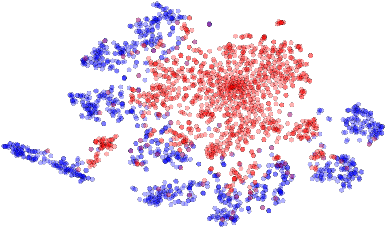
\includegraphics[width=0.45\textwidth]{./figures/adaptation_vis/pool2_mnist2inv_before.pdf}}\hfill%
  \subfigure[Adapted]{%%
    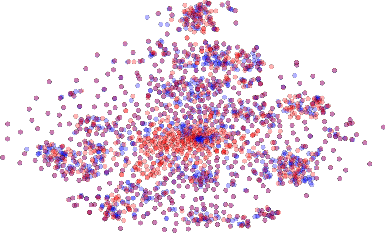
\includegraphics[width=0.45\textwidth]{./figures/adaptation_vis/pool2_mnist2inv_after.pdf}}%%
  \hspace*{\fill}%
  \end{minipage}%
  \begin{minipage}{.5\textwidth}
  \centering
  \small{{\sc Syn Numbers $ \rightarrow $ SVHN}: last hidden layer of the label predictor}
  \setcounter{subfigure}{0}
  \hspace*{\fill}%
  \subfigure[Non-adapted]{%%
    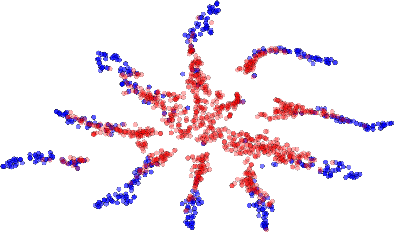
\includegraphics[width=0.45\textwidth]{./figures/adaptation_vis/before.pdf}}\hfill%
  \subfigure[Adapted]{%%
    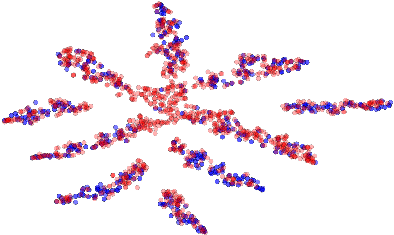
\includegraphics[width=0.45\textwidth]{./figures/adaptation_vis/after.pdf}}%%
  \hspace*{\fill}%
  \end{minipage}
  \caption{The effect of adaptation on the distribution of the extracted features (best viewed in color). The figure shows t-SNE \cite{Maaten13} visualizations of the CNN's activations {\bf (a)} in case when no adaptation was performed and {\bf (b)} in case when our adaptation procedure was incorporated into training. {\it Blue} points correspond to the source domain examples, while {\it red} ones correspond to the target domain. In all cases, the adaptation in our method makes the two distributions of features much closer.}
  \label{fig:exper_adapt_vis}
\end{figure*}

\subsection{Results}
\label{sect:exper_quant}

We now discuss the experimental settings and the results. In each case, we train on the source dataset and test on a different target domain dataset, with considerable shifts between domains (see \fig{exper_domains_examples}). The results are summarized in \tab{results} and \tab{results_office}. 

\vspace{2mm}\noindent {\bf MNIST $ \rightarrow $ MNIST-M.}
Our first experiment deals with the MNIST dataset~\cite{LeCun98} (source). In order to obtain the target domain ({\sc MNIST-M}) we blend digits from the original set over patches randomly extracted from color photos from BSDS500 \cite{Arbelaez11}. This operation is formally defined for two images $ I^{1}, I^{2} $ as $ I_{ijk}^{out} = | I_{ijk}^{1} - I_{ijk}^{2} | $, where $ i, j $ are the coordinates of a pixel and $ k $ is a channel index. In other words, an output sample is produced by taking a patch from a photo and inverting its pixels at positions corresponding to the pixels of a digit. For a human the classification task becomes only slightly harder compared to the original dataset (the digits are still clearly distinguishable) whereas for a CNN trained on MNIST this domain is quite distinct, as the background and the strokes are no longer constant. Consequently, the source-only model performs poorly. Our approach succeeded at aligning feature distributions (\fig{exper_adapt_vis}), which led to successful adaptation results (considering that the adaptation is unsupervised). At the same time, the improvement over source-only model achieved by subspace alignment (SA) \cite{Fernando13} is quite modest, thus highlighting the difficulty of the adaptation task. 

\vspace{2mm}\noindent {\bf Synthetic numbers $ \rightarrow $ SVHN.}
To address a common scenario of training on synthetic data and testing on  real data, we use Street-View House Number dataset {\sc SVHN} \cite{Netzer11} as the target domain and synthetic digits as the source. The latter ({\sc Syn ~Numbers}) consists of ~500,000 images generated by ourselves from Windows fonts by varying the text (that includes different one-, two-, and three-digit numbers), positioning, orientation, background and stroke colors, and the amount of blur. The degrees of variation were chosen manually to simulate SVHN, however the two datasets are still rather distinct, the biggest difference being the structured clutter in the background of SVHN images. 

The proposed backpropagation-based technique works well covering two thirds of the gap between training with source data only and training on target domain data with known target labels. In contrast, SA~\cite{Fernando13} does not result in any significant improvement in the classification accuracy, thus highlighting that the adaptation task is even more challenging than in the case of the MNIST experiment.

\vspace{2mm}\noindent {\bf MNIST $ \leftrightarrow $ SVHN.}
In this experiment, we further increase the gap between distributions, and test on {\sc MNIST} and {\sc SVHN}, which are significantly different in appearance. Training on SVHN even without adaptation is challenging --- classification error stays high during the first 150 epochs. In order to avoid ending up in a poor local minimum we, therefore, do not use learning rate annealing here. Obviously, the two directions ({\sc MNIST} $ \rightarrow $ {\sc SVHN} and {\sc SVHN} $ \rightarrow $ {\sc MNIST}) are not equally difficult. As {\sc SVHN} is more diverse, a model trained on SVHN is expected to be more generic and to perform reasonably on the MNIST dataset. This, indeed, turns out to be the case and is supported by the appearance of the feature distributions. We observe a quite strong separation between the domains when we feed them into the CNN trained solely on { \sc MNIST}, whereas for the {\sc SVHN}-trained network the features are much more intermixed. This difference probably explains why our method succeeded in improving the performance by adaptation in the {\sc SVHN} $ \rightarrow $ {\sc MNIST} scenario (see \tab{results}) but not in the opposite direction (SA is not able to perform adaptation in this case either). Unsupervised adaptation from MNIST to SVHN gives a failure example for our approach (we are unaware of any unsupervised DA methods capable of performing such adaptation).

\vspace{2mm}\noindent {\bf Synthetic Signs $ \rightarrow $ GTSRB.}
Overall, this setting is similar to the {\sc Syn Numbers} $ \rightarrow $ {\sc SVHN} experiment, except the distribution of the features is more complex due to the significantly larger number of classes (43 instead of 10). For the source domain we obtained~100,000 synthetic images (which we call {\sc Syn~Signs}) simulating various photoshooting conditions. Once again, our method achieves a sensible increase in performance once again proving its suitability for the synthetic-to-real data adaptation.

\begin{figure}
  \centering
  \setlength\figureheight{2.7cm}
  \setlength\figurewidth{6.8cm}
  % This file was created by matlab2tikz v0.5.0 running on MATLAB 8.3.
%Copyright (c) 2008--2014, Nico Schlömer <nico.schloemer@gmail.com>
%All rights reserved.
%Minimal pgfplots version: 1.3
%
%The latest updates can be retrieved from
%  http://www.mathworks.com/matlabcentral/fileexchange/22022-matlab2tikz
%where you can also make suggestions and rate matlab2tikz.
%
\begin{tikzpicture}[font=\scriptsize]

\begin{axis}[%
width=0.95092\figurewidth,
height=\figureheight,
at={(0\figurewidth,0\figureheight)},
scale only axis,
xmin=10000,
xmax=50000,
xlabel={Batches seen},
ymin=0,
ymax=1,
ylabel={Validation error},
axis x line*=bottom,
axis y line*=left,
legend style={at={($ (1,1) + (-0.1cm,-0.1cm) $)},anchor=north east,align=left,legend cell align=left,draw=black},
xmajorgrids,
ymajorgrids,
grid style={dashed}
]
\addplot [color=blue,solid,line width=1.0pt]
  table[row sep=crcr]{%
10500	0.199757996632997\\
11000	0.19162984006734\\
11500	0.190788089225589\\
12000	0.192918771043771\\
12500	0.196390993265993\\
13000	0.185527146464646\\
13500	0.190472432659933\\
14000	0.185606060606061\\
14500	0.183422769360269\\
15000	0.189051978114478\\
15500	0.191524621212121\\
16000	0.186079545454545\\
16500	0.179424452861953\\
17000	0.187684132996633\\
17500	0.187868265993266\\
18000	0.180923821548822\\
18500	0.187315867003367\\
19000	0.178661616161616\\
19500	0.18102904040404\\
20000	0.180555555555556\\
20500	0.176662457912458\\
21000	0.183791035353535\\
21500	0.179214015151515\\
22000	0.178898358585859\\
22500	0.178898358585859\\
23000	0.174479166666667\\
23500	0.174742213804714\\
24000	0.171059553872054\\
24500	0.177951388888889\\
25000	0.174794823232323\\
25500	0.174084595959596\\
26000	0.174636994949495\\
26500	0.169034090909091\\
27000	0.171191077441077\\
27500	0.170875420875421\\
28000	0.171506734006734\\
28500	0.170217803030303\\
29000	0.169244528619529\\
29500	0.169875841750842\\
30000	0.168744739057239\\
30500	0.17048085016835\\
31000	0.169454966329966\\
31500	0.167771464646465\\
32000	0.168849957912458\\
32500	0.168323863636364\\
33000	0.168718434343434\\
33500	0.165667087542088\\
34000	0.167376893939394\\
34500	0.169007786195286\\
35000	0.167140151515152\\
35500	0.165667087542088\\
36000	0.167850378787879\\
36500	0.169823232323232\\
37000	0.170691287878788\\
37500	0.16640361952862\\
38000	0.167981902356902\\
38500	0.169875841750842\\
39000	0.166771885521886\\
39500	0.169376052188552\\
40000	0.168087121212121\\
40500	0.165509259259259\\
41000	0.167718855218855\\
41500	0.168060816498317\\
42000	0.166035353535354\\
42500	0.166692971380471\\
43000	0.166429924242424\\
43500	0.167034932659933\\
44000	0.170349326599327\\
44500	0.169744318181818\\
45000	0.168218644781145\\
45500	0.166429924242424\\
46000	0.166324705387205\\
46500	0.168771043771044\\
47000	0.168034511784512\\
47500	0.168718434343434\\
48000	0.171059553872054\\
48500	0.170638678451178\\
49000	0.16819234006734\\
49500	0.168981481481481\\
50000	0.167902988215488\\
};
\addlegendentry{Real data only};

\addplot [color=cyan,solid,line width=1.0pt]
  table[row sep=crcr]{%
10500	0.9625\\
11000	0.79765625\\
11500	0.715625\\
12000	0.6140625\\
12500	0.52109375\\
13000	0.459375\\
13500	0.4484375\\
14000	0.421875\\
14500	0.39453125\\
15000	0.4109375\\
15500	0.34296875\\
16000	0.36875\\
16500	0.3359375\\
17000	0.36171875\\
17500	0.3171875\\
18000	0.3484375\\
18500	0.32421875\\
19000	0.315625\\
19500	0.346875\\
20000	0.31875\\
20500	0.35390625\\
21000	0.3265625\\
21500	0.33359375\\
22000	0.3171875\\
22500	0.28515625\\
23000	0.30546875\\
23500	0.309375\\
24000	0.2796875\\
24500	0.30859375\\
25000	0.30703125\\
25500	0.3078125\\
26000	0.28671875\\
26500	0.2875\\
27000	0.31484375\\
27500	0.2859375\\
28000	0.29375\\
28500	0.31328125\\
29000	0.3078125\\
29500	0.2859375\\
30000	0.2890625\\
30500	0.284375\\
31000	0.2953125\\
31500	0.26953125\\
32000	0.29921875\\
32500	0.30078125\\
33000	0.2640625\\
33500	0.309375\\
34000	0.2734375\\
34500	0.290625\\
35000	0.26796875\\
35500	0.3015625\\
36000	0.26796875\\
36500	0.2921875\\
37000	0.265625\\
37500	0.2765625\\
38000	0.2859375\\
38500	0.32109375\\
39000	0.28046875\\
39500	0.275\\
40000	0.24921875\\
40500	0.29140625\\
41000	0.26640625\\
41500	0.265625\\
42000	0.259375\\
42500	0.2765625\\
43000	0.26796875\\
43500	0.2765625\\
44000	0.27265625\\
44500	0.25546875\\
45000	0.26484375\\
45500	0.271875\\
46000	0.2703125\\
46500	0.26171875\\
47000	0.246875\\
47500	0.25078125\\
48000	0.29609375\\
48500	0.2640625\\
49000	0.26875\\
49500	0.26015625\\
50000	0.2578125\\
};
\addlegendentry{Synthetic data only};

\addplot [color=red,solid,line width=1.0pt]
  table[row sep=crcr]{%
10500	0.943892045454545\\
11000	0.943892045454545\\
11500	0.943892045454545\\
12000	0.943892045454545\\
12500	0.848300715488216\\
13000	0.658722643097643\\
13500	0.590593434343434\\
14000	0.475484006734007\\
14500	0.313946759259259\\
15000	0.235690235690236\\
15500	0.17879313973064\\
16000	0.152383207070707\\
16500	0.12912984006734\\
17000	0.114478114478114\\
17500	0.116214225589226\\
18000	0.1015625\\
18500	0.10066813973064\\
19000	0.101983375420875\\
19500	0.0914351851851852\\
20000	0.0895675505050505\\
20500	0.0894360269360269\\
21000	0.0827283249158249\\
21500	0.0798611111111111\\
22000	0.0859638047138047\\
22500	0.0799137205387205\\
23000	0.0778619528619529\\
23500	0.0737584175084175\\
24000	0.0742582070707071\\
24500	0.0776778198653199\\
25000	0.0771517255892256\\
25500	0.0725747053872054\\
26000	0.0739425505050505\\
26500	0.0734953703703704\\
27000	0.0730744949494949\\
27500	0.0688920454545455\\
28000	0.0702072811447811\\
28500	0.072337962962963\\
29000	0.0670244107744108\\
29500	0.0733638468013468\\
30000	0.0667613636363636\\
30500	0.0692340067340067\\
31000	0.0652093855218855\\
31500	0.0664720117845118\\
32000	0.0655776515151515\\
32500	0.0671296296296296\\
33000	0.0656039562289562\\
33500	0.0646043771043771\\
34000	0.0668665824915825\\
34500	0.0638678451178451\\
35000	0.065077861952862\\
35500	0.0649989478114478\\
36000	0.0672348484848485\\
36500	0.0668665824915825\\
37000	0.0626052188552189\\
37500	0.0652093855218855\\
38000	0.0626315235690236\\
38500	0.0627893518518518\\
39000	0.0613162878787879\\
39500	0.063236531986532\\
40000	0.0629208754208754\\
40500	0.0639467592592593\\
41000	0.0612899831649832\\
41500	0.0653409090909091\\
42000	0.0608691077441077\\
42500	0.0613425925925926\\
43000	0.0630260942760943\\
43500	0.060106271043771\\
44000	0.0638678451178451\\
44500	0.0602377946127946\\
45000	0.0577388468013468\\
45500	0.062684132996633\\
46000	0.0608164983164983\\
46500	0.0603167087542088\\
47000	0.0577651515151515\\
47500	0.0583175505050505\\
48000	0.0591329966329966\\
48500	0.0607112794612795\\
49000	0.0585805976430976\\
49500	0.0583175505050505\\
50000	0.0590540824915825\\
};
\addlegendentry{Both};

\end{axis}
\end{tikzpicture}%
  \caption{Semi-supervised domain adaptation for the traffic signs. As labeled target domain data are shown to the method, it achieves significantly lower error than the model trained on target domain data only or on source domain data only. \vspace{-4mm}}
  \label{fig:exper_semi_test}
\end{figure}

As an additional experiment, we also evaluate the proposed algorithm for semi-supervised domain adaptation, i.e.\ when one is additionally provided with a small amount of labeled target data. For that purpose we split {\sc GTSRB} into the train set (1280 random samples with labels) and the validation set (the rest of the dataset). The validation part is used solely for the evaluation and does not participate in the adaptation. The training procedure changes slightly as the label predictor is now exposed to the target data. \fig{exper_semi_test} shows the change of the validation error throughout the training. While the graph clearly suggests that our method can be used in the semi-supervised setting, thorough verification of semi-supervised setting is left for future work.


\vspace{2mm}\noindent {\bf Office dataset.} 
We finally evaluate our method on {\sc Office} dataset, which is a collection of three distinct domains: {\sc Amazon}, {\sc DSLR}, and {\sc Webcam}. Unlike previously discussed datasets, {\sc Office} is rather small-scale with only 2817 labeled images spread across 31 different categories in the largest domain. The amount of available data is crucial for a successful training of a deep model, hence we opted for the fine-tuning of the CNN pre-trained on the ImageNet \cite{Jia14} as it is done in some recent DA works \cite{Donahue14,Tzeng14,Hoffman14}. We make our approach more comparable with \cite{Tzeng14} by using exactly the same network architecture replacing domain mean-based regularization with the domain classifier.

Following most previous works, we evaluate our method using 5 random splits for each of the 3 transfer tasks commonly used for evaluation. Our training protocol is close to \cite{Tzeng14,Saenko10,Gong12} as we use the same number of labeled source-domain images per category. Unlike those works and similarly to e.g.\ DLID~\cite{Chopra13} we use the whole unlabeled target domain (as the premise of our method is the abundance of unlabeled data in the target domain). Under this transductive setting, our method is able to improve previously-reported state-of-the-art accuracy for unsupervised adaptation very considerably (\tab{results_office}), especially in the most challenging {\sc Amazon} $ \rightarrow $ {\sc Webcam} scenario (the two domains with the largest domain shift).

\section{VQA Dataset Analysis}
\label{sec:analysis}
%\vspace{\sectionReduceBot}
%%%%%%%%%%%%%%%%%%%%%%%%%%%%%%%%%%%%%%%%%%%%%%%%%%%%%%%%%%%
%%%%%%%%%%%%%%%%%%%%%%%%%%%%%%%%%%%%%%%%%%%%%%%%%%%%%%%%%%%
\begin{figure*}[t]
\centering
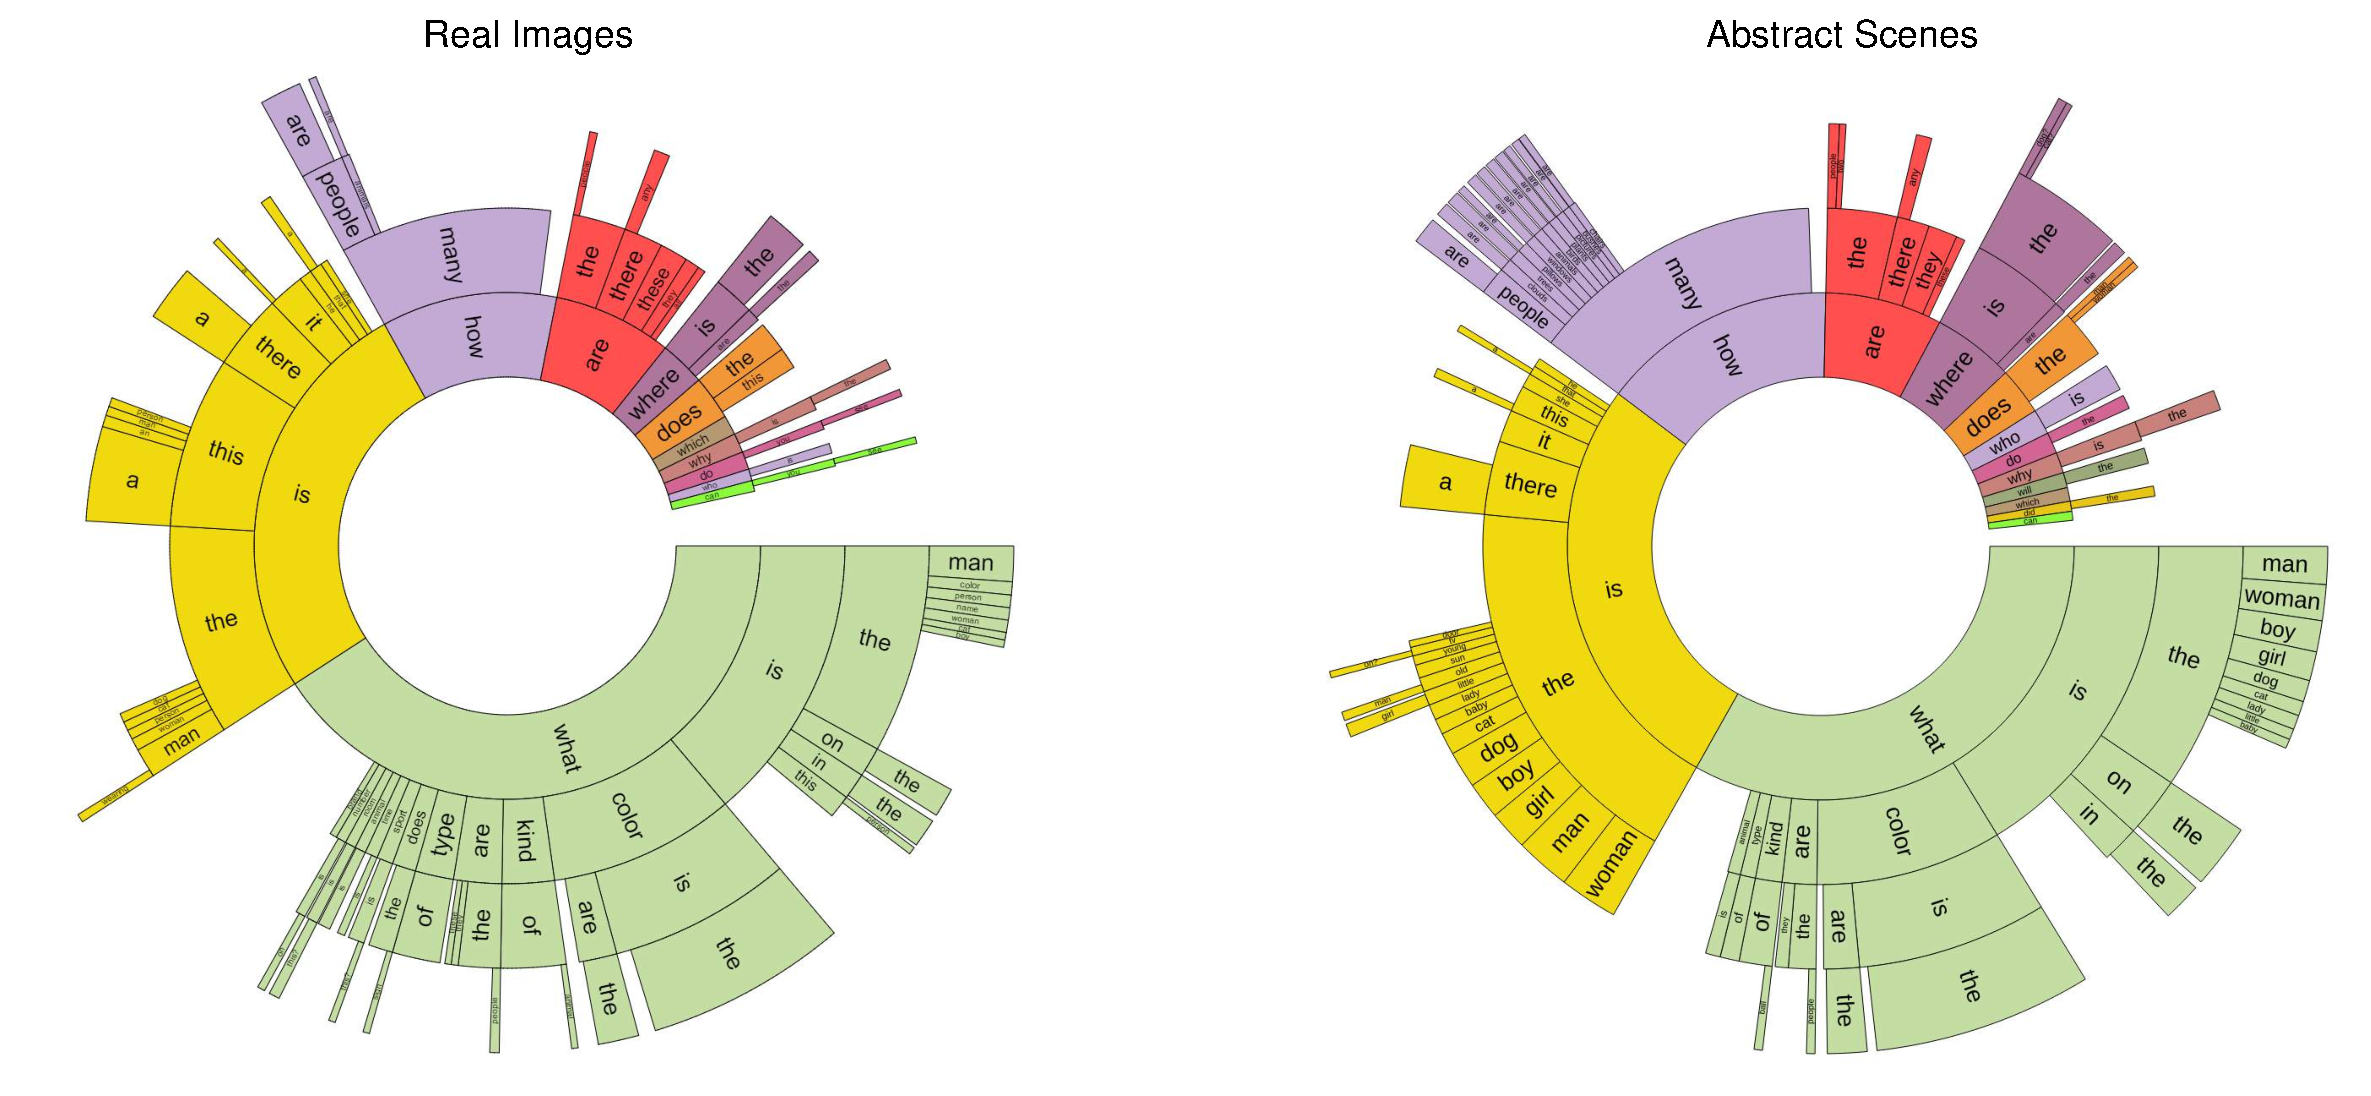
\includegraphics[width=1\linewidth]{figures/QuestionTypes3.pdf}
\caption{Distribution of questions by their first four words for a random sample of 60K questions for real images (left) and all questions for abstract scenes (right). The ordering of the words starts towards the center and radiates outwards. The arc length is proportional to the number of questions containing the word. White areas are words with contributions too small to show. }
%\vspace{-5pt}
\label{fig:QuesCluster}
%\setlength{\belowcaptionskip}{-10pt}
\end{figure*}
%%%%%%%%%%%%%%%%%%%%%%%%%%%%%%%%%%%%%%%%%%%%%%%%%%%%%%%%%%%

In this section, we provide an analysis of the questions and answers in the VQA train dataset.
To gain an understanding of the types of questions asked and answers provided, we visualize
the distribution of question types and answers. We also explore how often the questions may
be answered without the image using just commonsense information. Finally, we analyze whether
the information contained in an image caption is sufficient to answer the questions.

The dataset includes 614,163 questions 
%and a total of 
and 7,984,119 answers (including answers provided by workers with and without 
looking at the image) 
%and without looking at the image) 
for 204,721 images from the MS COCO dataset~\cite{coco} and 150,000 questions with 1,950,000 answers for $50,000$ abstract scenes.

%\textcolor{red}{
%We emphasize that the creation of a dataset of this scale and richness
%is a time consuming process, taking months to complete.
%While the entirety of the dataset has been collected,} at the time of original submission,
%120,520 questions with 270,210 answers for 50,000 MS COCO
%images and 30,000 questions with 79,740 answers for 10,000 abstract scenes had been collected.
%Please refer to the appendix for further details.
%\textcolor{red}{The results in this section still reflect that subset of the final dataset.}
%We emphasize that the creation of a dataset of this scale and richness
%is a time consuming process, taking months to complete.
%By our current estimates,
%approximately 5,000 questions and 40,000 answers are collected per day
%using Amazon Mechanical Turk (AMT).
%The entire dataset will take approximately three months to complete. At the time of submission,
%120,520 questions with 270,210 answers for 50,000 MS COCO
%images and 30,000 questions with 79,740 answers for 10,000 abstract scenes had been collected.
%Please refer to the appendix for further details.


%%%%%%%%%%%%%%%%%%%%%%%%%%%%%%%%%%%%%%%%%%%%%%%%%%%%%%%%%%%
%\vspace{\subsectionReduceTop}
\subsection{Questions}
%\vspace{\subsectionReduceBot}
%%%%%%%%%%%%%%%%%%%%%%%%%%%%%%%%%%%%%%%%%%%%%%%%%%%%%%%%%%%

\textbf{Types of Question.}
Given the structure of questions generated in the English language,
we can cluster questions into different types based on the words that start the question.
\figref{fig:QuesCluster} shows the distribution of questions based on the first four
words of the questions for both the real images (left) and abstract scenes (right).
Interestingly, the distribution of questions is quite similar for both real images and abstract scenes.
This helps demonstrate that the type of questions elicited by the abstract scenes is similar to
those elicited by the real images. There exists a surprising variety of question types,
including ``What is$\ldots$'', ``Is there$\ldots$'', ``How many$\ldots$'', and ``Does the$\ldots$''.
Quantitatively, the percentage of questions for different types is shown in \tableref{tab:typeacc}. Several example questions and answers are shown in \figref{fig:qualResults}.
%\textbf{Sub-Types.}
A particularly interesting type of question is the ``What is$\ldots$'' questions, since they have a
diverse set of possible answers. See the appendix for visualizations for ``What is$\ldots$'' questions.

\textbf{Lengths.}
\figref{fig:QuesLen} shows the distribution of question lengths.
We see that most questions range from four to ten words.


\begin{comment}\begin{table}[h]
{\small
\begin{tabular}{@{\extracolsep{\fill}}p{2cm}|ccccc@{\extracolsep{\fill}}}
%\toprule
Dataset  & Yes & No\\
%\midrule
Real   & 18.21 & 14.06 \\
Abstract & 26.54 & 16.70 \\
\end{tabular}
}
\vspace{5pt}
\caption{Percentage of ``yes'' and ``no'' questions in the real and abstract datasets.}
\label{table:yesno}
%\vspace{\captionReduceBot}
\end{table}
\end{comment}

%%%%%%%%%%%%%%%%%%%%%%%%%%%%%%%%%%%%%%%%%%%%%%%%%%%%%%%%%%%
\begin{figure}[t]
\centering
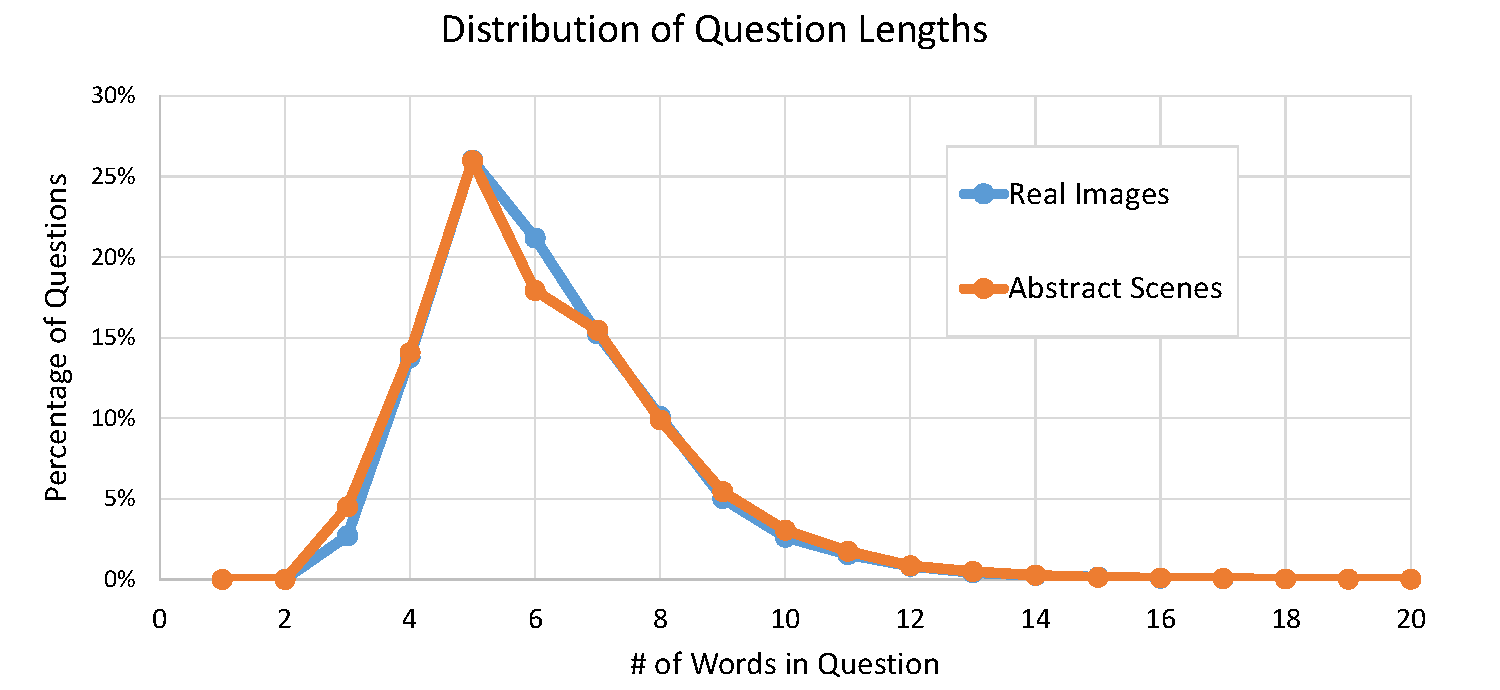
\includegraphics[width=1\linewidth]{figures/Lengths.pdf}
%\vspace{-9pt}
\caption{Percentage of questions with different word lengths for real images and abstract scenes.}
%\vspace{-5pt}
\label{fig:QuesLen}
%\setlength{\belowcaptionskip}{-10pt}
\end{figure}
%%%%%%%%%%%%%%%%%%%%%%%%%%%%%%%%%%%%%%%%%%%%%%%%%%%%%%%%%%%




\begin{figure*}
\centering
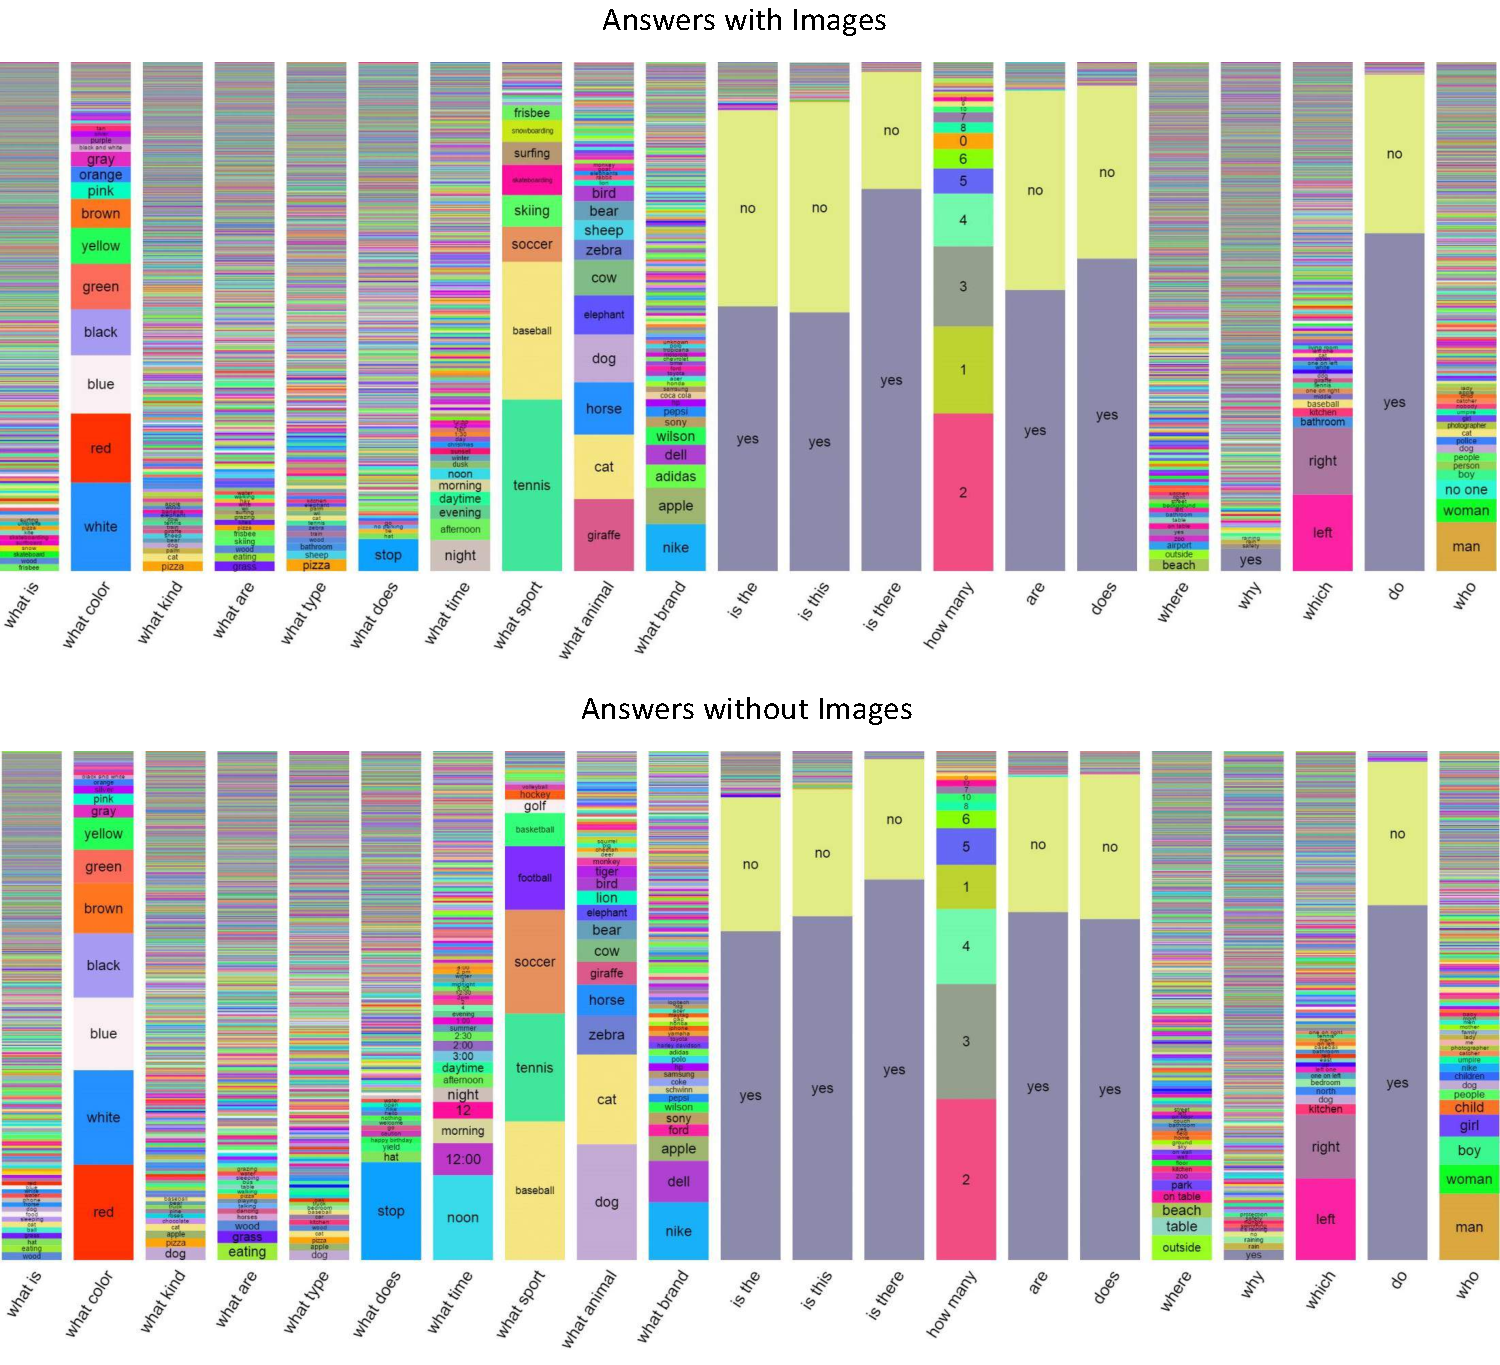
\includegraphics[width=1\linewidth]{figures/answers.pdf}
%\vspace{-5pt}
\caption{Distribution of answers per question type for a random sample of 60K questions for real images when subjects provide answers when given the image (top) and when not given the image (bottom).}
%\vspace{-5pt}
\label{fig:AnsPerQues}
%\setlength{\belowcaptionskip}{-10pt}
\end{figure*}


%%%%%%%%%%%%%%%%%%%%%%%%%%%%%%%%%%%%%%%%%%%%%%%%%%%%%%%%%%%
%\vspace{\subsectionReduceTop}
\subsection{Answers}
%\vspace{\subsectionReduceBot}
%%%%%%%%%%%%%%%%%%%%%%%%%%%%%%%%%%%%%%%%%%%%%%%%%%%%%%%%%%%

%\textbf{Typical Answers for Different Question Types.}
\textbf{Typical Answers.}
%Next, we analyze the answers provided for different question types.
\figref{fig:AnsPerQues} (top) shows the distribution of answers for several question types.
We can see that a number of question types, such as ``Is the\ldots'', ``Are\ldots'', and ``Does\ldots'' are
typically answered using ``yes'' and ``no'' as answers.
%\textcolor{red}{Question types such as ``How many\ldots'' are answered using numbers. $12.31\%$ and $14.48\%$ of the questions are answered using numbers on real images and abstract scenes, respectively.}
Other questions such as ``What is\ldots'' and ``What type\ldots'' have a rich diversity
of responses. Other question types such as ``What color\ldots'' or ``Which\ldots'' have more specialized responses,
such as colors, or ``left'' and ``right''. 
See the appendix for a list of the most popular answers.

\textbf{Lengths.}
Most answers consist of a single word, with the distribution of answers containing one, two, or three words, respectively being $89.32\%$, $6.91\%$, and $2.74\%$ for real images and $90.51\%$, $5.89\%$, and $2.49\%$ for abstract scenes.
%$89.16\%$, $7.00\%$, and $2.77\%$ of answers containing one, two, or three words, respectively.
The brevity of answers is not surprising, since the questions tend to elicit specific
information from the images. This is in contrast with image captions that generically
describe the entire image and hence tend to be longer. The brevity of our answers makes
automatic evaluation feasible. While it may be tempting to believe the brevity of the answers
makes the problem easier, recall that they are human-provided open-ended answers to
open-ended questions. The questions typically require complex reasoning to arrive at these
deceptively simple answers (see \figref{fig:qualResults}).
There are currently 23,234 unique one-word answers in our dataset for real images and 3,770 for abstract scenes.
%There are currently 10,011 unique one-word answers in our dataset.

\textbf{`Yes/No' and `Number' Answers.}
Many questions are answered using either ``yes'' or ``no'' (or sometimes ``maybe'') -- 
$38.37\%$ and $40.66\%$ of the questions on real images and abstract scenes respectively. 
Among these `yes/no' questions, there is a bias towards %answering with 
``yes'' -- %with ``yes'' being preferred %$61.32\%$ and $58.46\%$ 
$58.83\%$ and $55.86\%$ of `yes/no' answers are ``yes'' for real images and abstract scenes. 
Question types such as ``How many\ldots'' are answered using numbers -- 
$12.31\%$ and $14.48\%$ of the questions on real images and abstract scenes are `number' questions. 
``2'' is the most popular answer among the `number' questions, making up 
$26.04\%$ of the `number' answers for real images and $39.85\%$ for abstract scenes. 

\textbf{Subject Confidence.}
When the subjects answered the questions, we asked
``Do you think you were able to answer the question correctly?''.
\figref{fig:ConfScores} shows the distribution of responses. A majority of the answers
were labeled as confident for both real images and abstract scenes. % respectively.

\textbf{Inter-human Agreement.}
Does the self-judgment of confidence correspond to the answer agreement between subjects?
\figref{fig:ConfScores} shows the percentage of questions in which 
(i) $7$ or more, 
(ii) $3-7$, or 
(iii) less than $3$ subjects agree on the answers given their average confidence score 
(0 = not confident, 1 = confident).
As expected, the agreement between subjects increases with confidence.
However, even if all of the subjects are confident the answers may still vary.
This is not surprising since some answers may vary, yet have very similar meaning, such as ``happy'' and ``joyful''.

\begin{figure}[t]
\centering
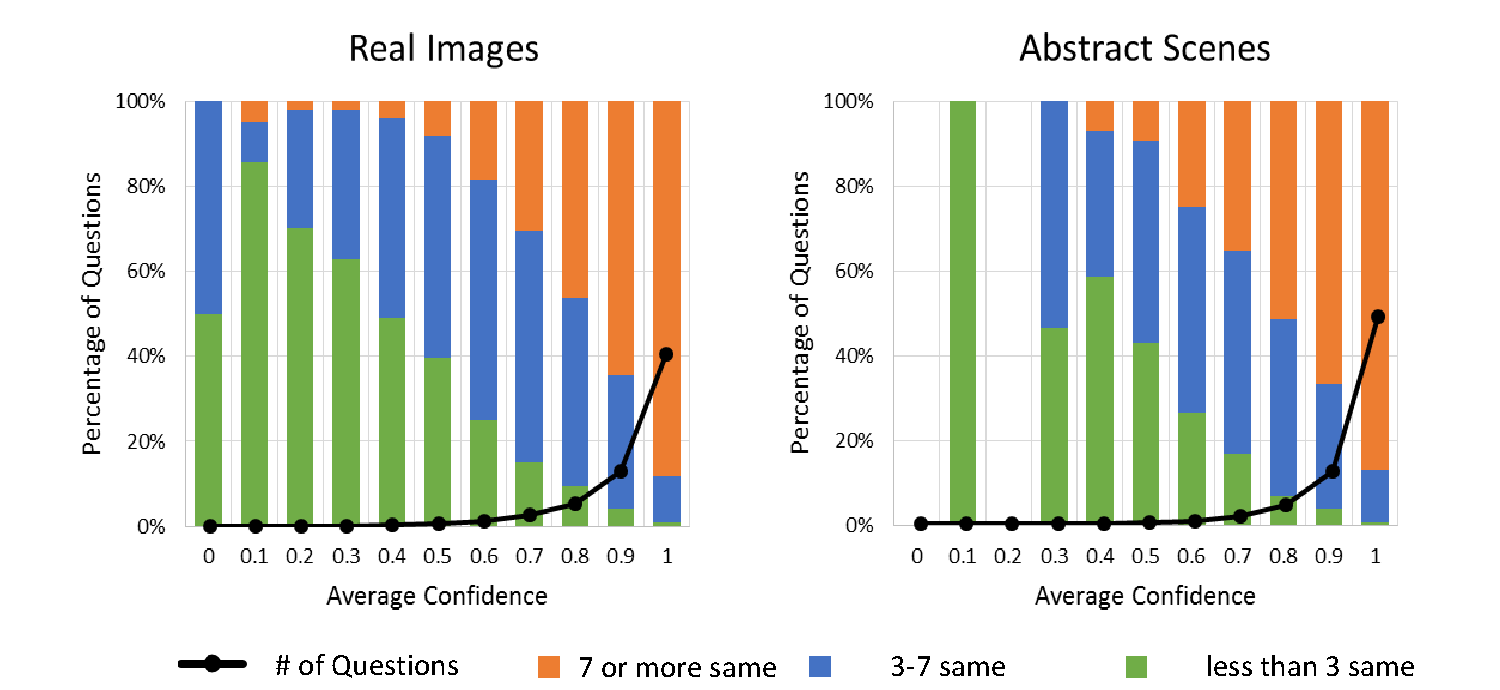
\includegraphics[width=1\linewidth]{figures/Confidence.pdf}
%\vspace{-5pt}
\caption{Number of questions per average confidence score (0 = not confident, 1 = confident) for real images and abstract scenes (black lines). Percentage of questions where 7 or more answers are same, 3-7 are same, less than 3 are same (color bars). }
%\vspace{-7pt}
\label{fig:ConfScores}
%\setlength{\belowcaptionskip}{-10pt}
\end{figure}

As shown in \tableref{table:commonsense_acc} (Question + Image), there is significant inter-human
agreement in the answers for both real images ($83.30\%$) and abstract scenes ($87.49\%$). 
%when humans are provided both the question and image while answering the question.
Note that on average each question has $2.70$ unique answers for real images and $2.39$ for abstract scenes. 
The agreement is significantly higher ($>95\%$) for \quotes{yes/no} questions and lower for other questions ($<76\%$), possibly due to the fact that we perform exact string matching and do not account for synonyms, plurality, \etc. Note that the automatic determination of synonyms is a difficult problem, since the level of answer granularity can vary across questions.




%%%%%%%%%%%%%%%%%%%%%%%%%%%%%%%%%%%%%%%%%%%%%%%%%%%%%%%%%%%
%\vspace{\subsectionReduceTop}
\subsection{Commonsense Knowledge}
\label{sec:cs}
%\vspace{\subsectionReduceBot}
%%%%%%%%%%%%%%%%%%%%%%%%%%%%%%%%%%%%%%%%%%%%%%%%%%%%%%%%%%%
\begin{figure*}[t]
 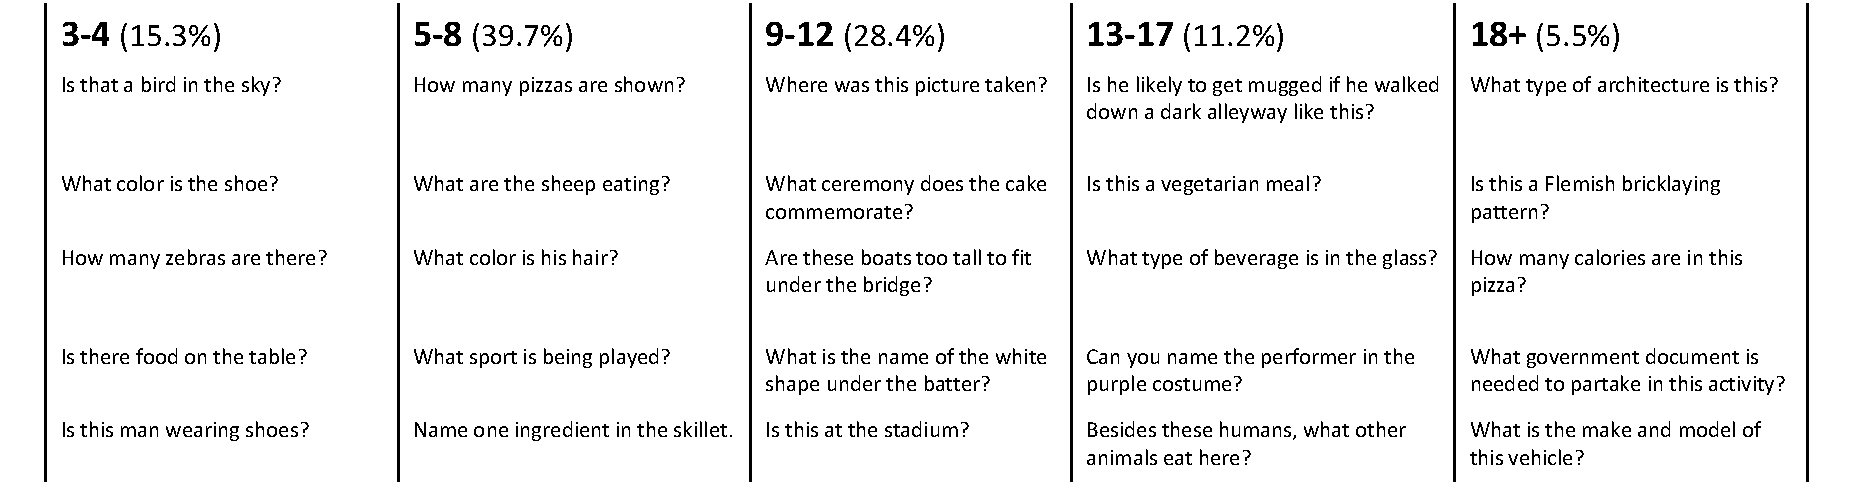
\includegraphics[width=\linewidth]{figures/age.pdf}
 \centering
\caption{\small Example questions judged by Mturk workers to be answerable by different age groups. The percentage of questions falling into each age group is shown in parentheses.}
 \label{fig:age}
 \end{figure*}
 	
\textbf{Is the Image Necessary?}
%Can the questions be answered using commonsense knowledge alone without the need for an image,
%\eg, ``What is the color of the sheep?''?
Clearly, some questions can sometimes be
answered correctly using commonsense knowledge alone without the need for an image,
\eg, ``What is the color of the fire hydrant?''.
We explore this issue by asking three subjects to answer
the questions \emph{without seeing the image} (see the examples in blue in \figref{fig:qualResults}).
In \tableref{table:commonsense_acc} (Question), we show the percentage of questions for which
the correct answer is provided over all questions, ``yes/no'' questions, and the other questions that
are not ``yes/no''. For ``yes/no'' questions, the human subjects respond better than chance.
For other questions, humans are only correct about $21\%$ of the time. This demonstrates that
understanding the visual information is critical to VQA and that commonsense information alone is not sufficient.

To show the qualitative difference in answers provided with and without images,
we show the distribution of answers for various question types in \figref{fig:AnsPerQues} (bottom).
The distribution of colors, numbers, and even ``yes/no'' responses is surprisingly different for answers
with and without images.
 
\textbf{Which Questions Require Common Sense?}
In order to identify questions that require commonsense reasoning to answer, we conducted 
two AMT studies (on a subset 10K questions from the real images of VQA trainval) asking subjects --
\begin{compactenum} 
\item Whether or not they believed a question required commonsense to answer the question, and 
\item The youngest age group that they believe a person must be in order to be able to correctly answer the question -- 
toddler (3-4), 
younger child (5-8), 
older child (9-12), 
teenager (13-17), 
adult (18+).
\end{compactenum}
Each question was shown to 10 subjects. We found that 
for $47.43\%$ of questions 3 or more subjects voted `yes' to commonsense, 
($18.14\%$: 6 or more).  
In the `perceived human age required to answer question' study, we found the following distribution of responses: 
toddler: $15.3\%$,
younger child: $39.7\%$, 
older child: $28.4\%$, 
teenager: $11.2\%$, 
adult: $5.5\%$.
In Figure \ref{fig:age} we show several questions for which a majority of subjects picked the specified age range. Surprisingly the perceived age needed to answer the questions is fairly well distributed across the different age ranges. As expected the questions that were judged answerable by an adult (18+) generally need specialized knowledge, whereas those answerable by a toddler (3-4) are more generic.
 
We measure the degree of commonsense required to answer a question as the percentage of subjects (out of 10) who voted ``yes'' in our ``whether or not a question requires commonsense'' study.
A fine-grained breakdown of average age and average degree of common sense (on a scale of $0-100$) required to answer a question is shown in \tableref{tab:typeacc}. The average age and the average degree of commonsense across all questions is $8.92$ and $31.01\%$ respectively. 

%\arxiv{To compute average age and average degree of commonsense across questions, we first compute the average age and average degree of commonsense (binary response scaled to $0-100$) per question (by taking average across 10 subjects for each question) and then take average across questions.} 

It is important to distinguish between:
\begin{compactenum}
\item How old someone needs to be to be able to answer a question correctly,  and
\item How old people \emph{think} someone needs to be to be able to answer a question correctly. 
\end{compactenum}

Our age annotations capture the latter -- perceptions of MTurk workers in an uncontrolled environment. As such, the relative ordering of question types in \tableref{tab:typeacc} is more important than absolute age numbers.
%The relative ordering of question types is more important than the absolute age numbers. It is important to note that the age annotations we have collected are just perceived ages: how old people -- untrained MTurk workers in an uncontrolled environment -- \emph{think} someone needs to be to be able to answer a question correctly.}
The two rankings of questions in terms of common sense required according to the two studies 
were largely correlated (Pearson's rank correlation: 0.58). 

%%%%%%%%%%%%%%%%%%%%%%%%%%%%%%%%%%%%%%%%%%%%%%%%%%%%%%%%%%%
\begin{table}[t]
\setlength{\tabcolsep}{3.2pt}
{\small
\begin{center}
%\begin{tabular}{@{}llccc@{}}
%\toprule
%Dataset & Input & All & Yes/No & Other \\
%%\hline
%\midrule
%    & Question & 40.81 & 67.60 & 21.22 \\
%Real   & Question + Caption* & 57.47 & 78.97 & 44.41 \\
%    & Question + Image & 83.30 & 95.77 & 72.67 \\
%%\hline
%\midrule
% & Question & 43.27 & 66.65 &  23.66 \\
%Abstract & Question + Caption* & 54.34 & 74.70 & 40.18 \\
% & Question + Image & 87.49 & 95.96 & 75.33 \\
%\bottomrule
%\end{tabular}
\begin{tabular}{@{}llcccc@{}}
\toprule
Dataset & Input & All & Yes/No & Number & Other \\
%\hline
\midrule
    & Question & 40.81 & 67.60 & 25.77 & 21.22 \\
Real   & Question + Caption* & 57.47 & 78.97 & 39.68 & 44.41 \\
    & Question + Image & 83.30 & 95.77 & 83.39 & 72.67 \\
%\hline
\midrule
 & Question & 43.27 & 66.65 & 28.52 & 23.66 \\
Abstract & Question + Caption* & 54.34 & 74.70 & 41.19 & 40.18 \\
 & Question + Image & 87.49 & 95.96 & 95.04 & 75.33 \\
\bottomrule
\end{tabular}
\end{center}
}
%\vspace{-7pt}
\caption {Test-standard accuracy of human subjects when asked to answer the 
question without seeing the image (Question), 
seeing just a caption of the image and not the image itself (Question + Caption), 
and seeing the image (Question + Image). 
Results are shown for all questions, ``yes/no'' \& ``number'' questions, and other questions 
that are neither answered ``yes/no'' nor number. 
All answers are free-form and not multiple-choice. 
*\hspace{1pt}These accuracies are evaluated on a subset of 3K train questions (1K images).}
% \textcolor{red}{and are not directly comparable to the corresponding numbers in older version.}}
\label{table:commonsense_acc}
%\vspace{\captionReduceBot}
%\vspace{-5pt}
\end{table}
%%%%%%%%%%%%%%%%%%%%%%%%%%%%%%%%%%%%%%%%%%%%%%%%%%%%%%%%%%%


%%%%%%%%%%%%%%%%%%%%%%%%%%%%%%%%%%%%%%%%%%%%%%%%%%%%%%%%%%%
%\vspace{\subsectionReduceTop}
\subsection{Captions \textbf{\vs} Questions}
%\vspace{\subsectionReduceBot}
%%%%%%%%%%%%%%%%%%%%%%%%%%%%%%%%%%%%%%%%%%%%%%%%%%%%%%%%%%%


Do generic image captions provide enough information to answer the questions?
\tableref{table:commonsense_acc} (Question + Caption) shows the percentage of questions answered
correctly when human subjects are given the question and a human-provided caption
describing the image, but not the image. As expected, the results are better than when humans are shown the questions alone.
However, the accuracies are significantly lower than when subjects are shown the actual image.
This demonstrates that in order to answer the questions correctly, deeper image understanding 
(beyond what image captions typically capture) is necessary. In fact, we find that the distributions of nouns, verbs, and adjectives mentioned in captions is statistically significantly different from those mentioned in our questions + answers (Kolmogorov-Smirnov test, $p<.001$) for both real images and abstract scenes. See the appendix for details. 
%This motivates the VQA task as a way to learn further information about visual scenes.
\section{Discussion}
\label{sec:discussion}

The accuracy on the CKP set shows that the chosen approach is robust, misclassification usually occurs on pictures which are the first few instances of an emotion sequence. Often a neutral facial expression is depicted in those frames. Thus those misclassifications are not necessarily an error in the approach, but in the data selection. Other than that no major problem could be detected. The emotion \textit{Surprise} is often confused with \textit{Disgust} with a rate of 0.045\% which is the highest. Of those images, where an emotion is present, only few are wrongly classified.\\ 


As there is no consent for the misclassified images, they cannot be depicted here. However some unique names are provided. \\
Image S119\_001\_00000010 is classified as \textit{Fear} while the annotated emotion corresponds to \textit{Surprise}. The image depicts a person with a wide open mouth and open eyes. Pictures representing \textit{Surprise} are often very similar, since the persons also have wide open mouths and eyes. In image S032\_004\_00000014 the targeted label \textit{Fear} is confused with \textit{Anger}. While the mouth region in pictures with \textit{Anger} differ, the eye regions are alike, since in both situations the eyes and eyebrows are contracted.\\
Similar effects are experienced when dealing with the MMI Dataset. Since the first two frames are discarded most pictures with neutral positions are excluded. In few images a neutral position can still be found which gives rise to errors. For the same reason as the CKP set images will not be displayed. Due to the approach to extract images of the videos, a unique identifier for the misclassified image cannot be provided.\\
The top confusions are observed for \textit{Fear} and \textit{Surprise} with a rate of 0.0159\% where \textit{Fear} is wrongly misclassified as \textit{Surprise}. Session 1937 shows a woman displaying \textit{Fear} but it is classified as \textit{Surprise}. Both share common features like similar eye and mouth movement. In both emotions, participants move the head slightly backwards. This can be identified by wrinkled skin. The second most confusion rate, \textit{Surprise} being mistaken as \textit{Sadness}, is mostly based on neutral position images. Although the first two images are not used, some selected frames still do not contain an emotion. In Session 1985 \textit{Surprise} is being mistaken as \textit{Sadness}. The image depicts a man with his mouth being slightly curved, making him look sad.\\

DeXpression extracts features and uses them to classify images, but in very few cases the emotions are confused. This happens, as discussed, usually in pictures depicting no emotion. DeXpression performs very well on both tested sets, if an emotion is present.


\label{sec:conclusion}
We introduce a novel neural network architecture, the Synchronized Spectral CNN (SyncSpecCNN), for semantic annotation on 3D shape graphs. To share coefficients and conduct multi-scale analysis in different parts of a single shape graph, we introduce a spectral parametrization of dilated convolutional kernels. To allow parameter sharing across related but different shapes that may be represented by very different graphs, we introduce a spectral transformer network to synchronize different spectral domains. The effectiveness of different components in our network is validated through extensive experiments. Jointly these contributions lead to state-of-the-art performance on various semantic annotation tasks including 3D shape part segmentation and 3D keypoint prediction.


\section*{Acknowledgments}

We thank the anonymous reviewers for their thoughtful feedback. Stanford University gratefully acknowledges the support of the Defense Advanced Research Projects Agency (DARPA) Deep Exploration and Filtering of Text (DEFT) Program under Air Force Research Laboratory (AFRL) contract no. FA8750-13-2-0040. Any opinions, findings, and conclusion or recommendations expressed in this material are those of the authors and do not necessarily reflect the view of the DARPA, AFRL, or the US government.

\bibliography{refs}
\bibliographystyle{acl2016}

\appendix
\section{RNN Encoder--Decoder}
\label{sec:detail}

In this document, we describe in detail the architecture of the RNN
Encoder--Decoder used in the experiments.

Let us denote an source phrase by $X=\left( \vx_1, \vx_2, \dots, \vx_N \right)$
and a target phrase by $Y=\left( \vy_1, \vy_2, \dots, \vy_M \right)$. Each
phrase is a sequence of $K$-dimensional one-hot vectors, such that only one
element of the vector is $1$ and all the others are $0$. The index of the active
($1$) element indicates the word represented by the vector.

\subsection{Encoder}

Each word of the source phrase is embedded in a $500$-dimensional vector space:
$e(\vx_i) \in \RR^{500}$. $e(\vx)$ is used in Sec.~\ref{sec:rep} to visualize
the words.

The hidden state of an encoder consists of $1000$ hidden units,
and each one of them at time $t$ is computed by
\begin{align*}
    h_j^{\qt{t}} = z_j h_j^{\qt{t-1}} + (1 - z_j) \tilde{h}_j^{\qt{t}},
\end{align*}
where
\begin{align*}
    \tilde{h}_j^{\qt{t}} =& \tanh\left( \left[ \mW e(\vx_t) \right]_j + \left[
    \mU \left( \vr \odot \vh_{\qt{t-1}}\right) \right]_j \right),
    \\
    z_j =& \sigma\left( \left[ \mW_z e(\vx_t) \right]_j + 
    \left[\mU_z \vh_{\qt{t-1}}\right]_j \right),
    \\
    r_j =& \sigma\left( \left[ \mW_r e(\vx_t) \right]_j + 
    \left[\mU_r \vh_{\qt{t-1}}\right]_j \right).
\end{align*}
$\sigma$ and $\odot$ are a logistic sigmoid function and an element-wise
multiplication, respectively. To make the equations uncluttered, we omit
biases. The initial hidden state $h_j^{\qt{0}}$ is fixed to $0$.

Once the hidden state at the $N$ step (the end of the source
phrase) is computed, the representation of the source phrase
$\vc$ is
\begin{align*}
    \vc = \tanh \left( \mV \vh^{\qt{N}} \right).
\end{align*}

\subsubsection{Decoder}

The decoder starts by initializing the hidden state with
\begin{align*}
    {\vh'}^{\qt{0}} = \tanh \left( \mV' \vc \right),
\end{align*}
where we will use $\cdot'$ to distinguish parameters of the
decoder from those of the encoder.

The hidden state at time $t$ of the decoder is computed by
\begin{align*}
    {h'}_j^{\qt{t}} = {z'}_j {h'}_j^{\qt{t-1}} +
    (1 - {z'}_j) \tilde{h'}_j^{\qt{t}},
\end{align*}
where
\begin{align*}
    \tilde{h'}_j^{\qt{t}} =& \tanh\left( 
    \left[ \mW' e(\vy_{t-1}) \right]_j + 
    {r'}_j \left[ \mU' {\vh'}_{\qt{t-1}} +
    \mC \vc 
    \right]
    \right),
    \\
    {z'}_j =& \sigma\left( \left[ {\mW'}_z e(\vy_{t-1}) \right]_j + 
    \left[{\mU'}_z {\vh'}_{\qt{t-1}}\right]_j +
    \left[\mC_z \vc \right]_j 
    \right),
    \\
    {r'}_j =& \sigma\left( \left[ {\mW'}_r e(\vy_{t-1}) \right]_j + 
    \left[{\mU'}_r {\vh'}_{\qt{t-1}}\right]_j +
    \left[ \mC_r \vc \right]_j
    \right),
\end{align*}
and $e(\vy_{0})$ is an all-zero vector. Similarly to the case of
the encoder, $e(\vy)$ is an embedding of a target word.

Unlike the encoder which simply encodes the source phrase, the
decoder is learned to generate a target phrase. At each time $t$,
the decoder computes the probability of generating $j$-th word by
\begin{align*}
    p(y_{t,j} = 1 \mid \vy_{t-1}, \dots, \vy_1, X) = \frac{\exp
        \left( {\vg}_j \vs_{\qt{t}}\right) } {\sum_{j'=1}^{K}
        \exp \left( \vg_{j'} \vs_{\qt{t}}\right) },
\end{align*}
where the $i$-element of $\vs_{\qt{t}}$ is 
\begin{align*}
    s_i^{\qt{t}} = \max\left\{
    {s'}_{2i-1}^{\qt{t}}, {s'}_{2i}^{\qt{t}}
\right\}
\end{align*}
and
\begin{align*}
    {\vs'}^{\qt{t}} = \mO_h {\vh'}^{\qt{t}} + \mO_y \vy_{t-1} + \mO_c \vc.
\end{align*}
In short, the $s_i^{\qt{t}}$ is a so-called \textit{maxout} unit.

For the computational efficiency, instead of a single-matrix
output weight $\mG$, we use a product of two matrices such that
\begin{align*}
    \mG = \mG_l \mG_r,
\end{align*}
where $\mG_l \in \RR^{K \times 500}$ and $\mG_r \in \RR^{500 \times
1000}$.


\section{Word and Phrase Representations}
\label{sec:word_phrase_embed}

Here, we show enlarged plots of the word and phrase
representations in
Figs.~\ref{fig:word_embed}--\ref{fig:phrase_embed}.

\newpage
\begin{landscape}
\begin{figure*}[p]
    \iftoggle{arxiv}{
        \vspace{-20mm}
    }
    \centering
    \begin{minipage}{0.75\textwidth}
        \centering
        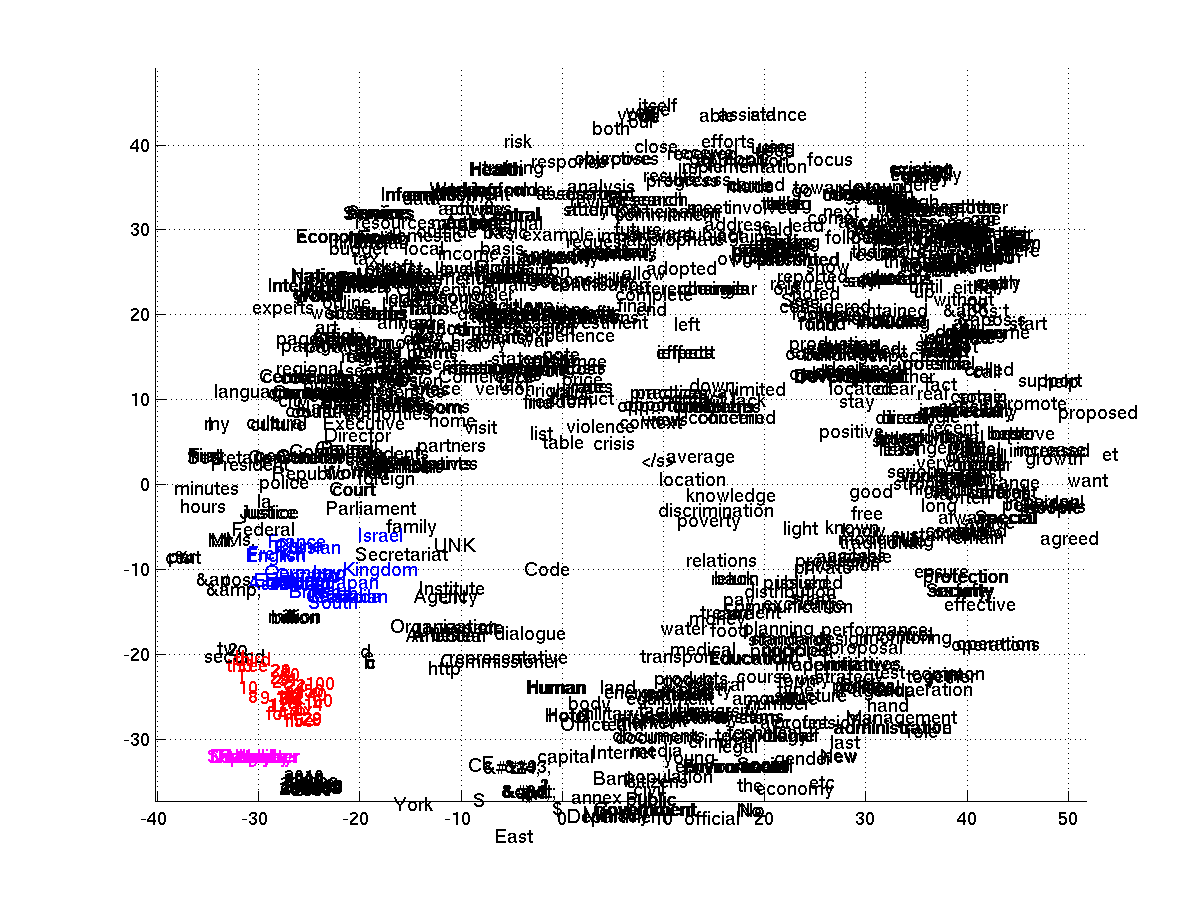
\includegraphics[width=0.99\textwidth]{word_all.png}
    \end{minipage}
    \begin{minipage}{0.75\textwidth}
        \centering
        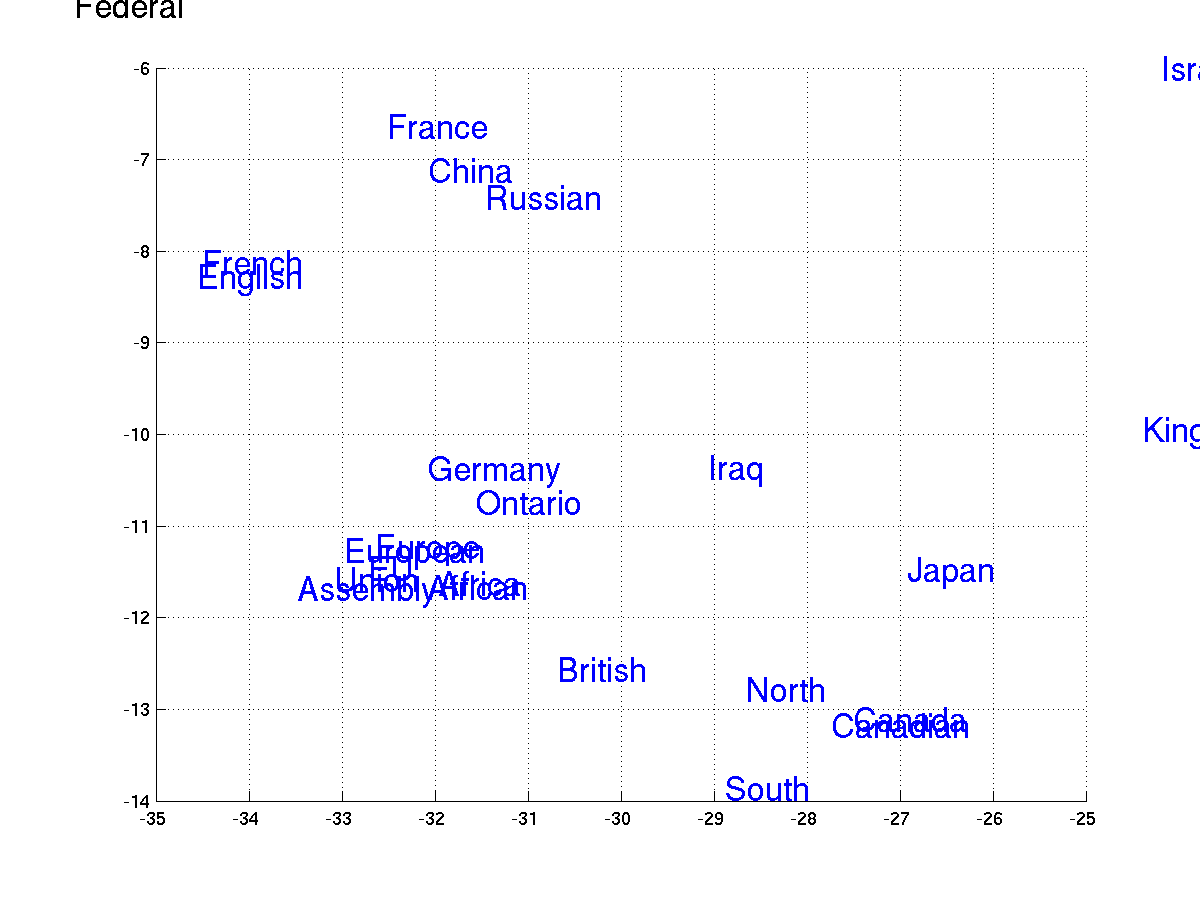
\includegraphics[width=0.99\textwidth]{word_countries.png}
    \end{minipage}
    \\
    \begin{minipage}{0.75\textwidth}
        \centering
        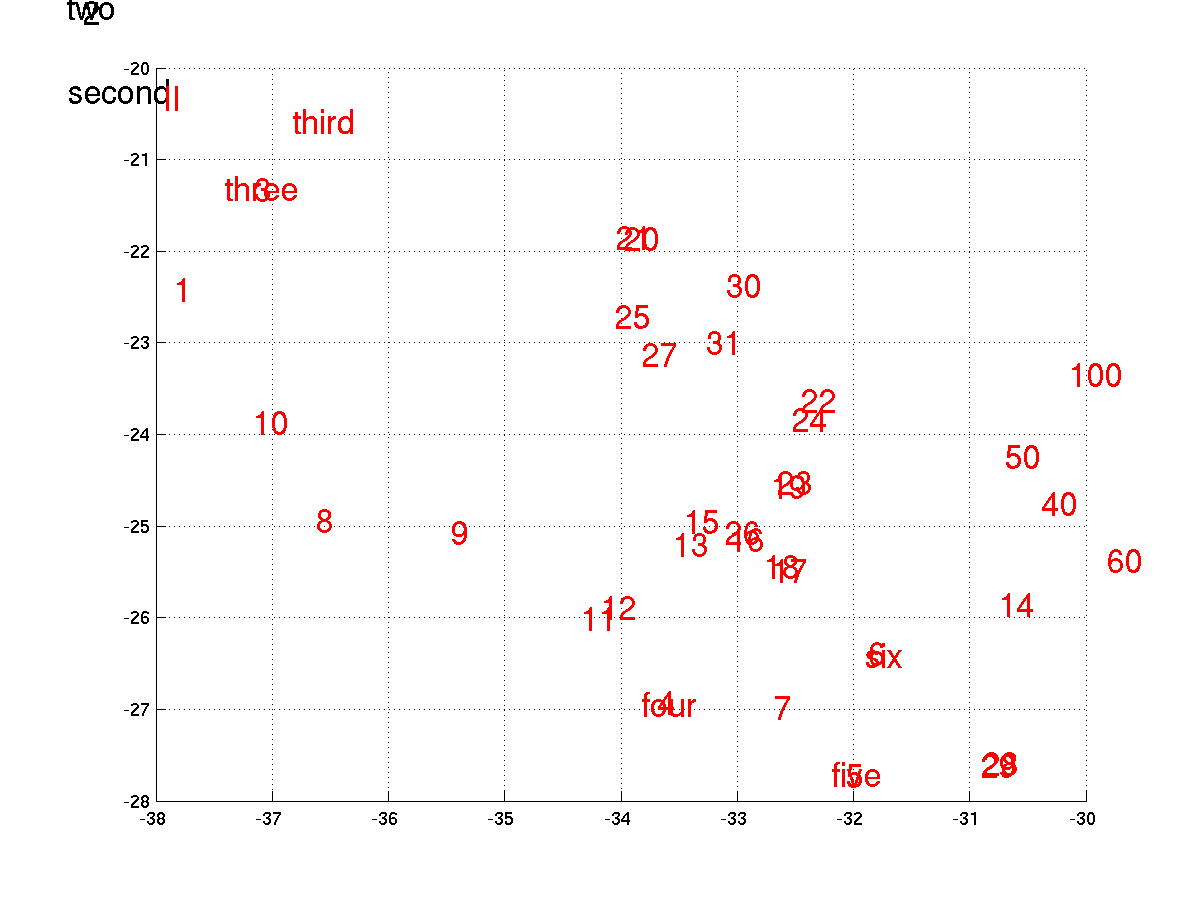
\includegraphics[width=0.99\textwidth]{word_numbers.png}
    \end{minipage}
    \begin{minipage}{0.75\textwidth}
        \centering
        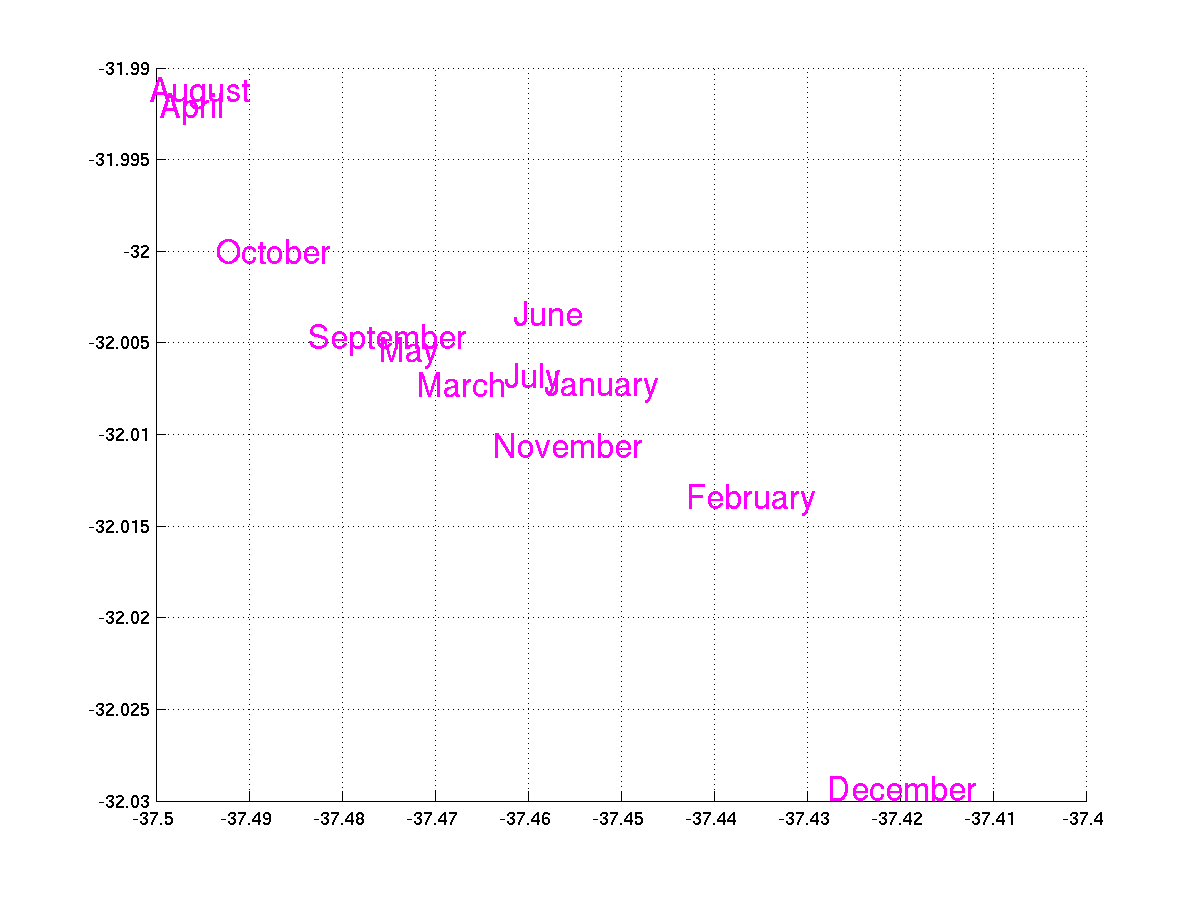
\includegraphics[width=0.99\textwidth]{word_months.png}
    \end{minipage}
    \caption{2--D embedding of the learned word representation. The top left one
        shows the full embedding space, while the other three figures show the
    zoomed-in view of specific regions (color--coded).} 
\end{figure*}
\end{landscape}


\newpage
\begin{landscape}
\begin{figure*}[p]
    \iftoggle{arxiv}{
        \vspace{-20mm}
    }
    \centering
    \begin{minipage}{0.75\textwidth}
        \centering
        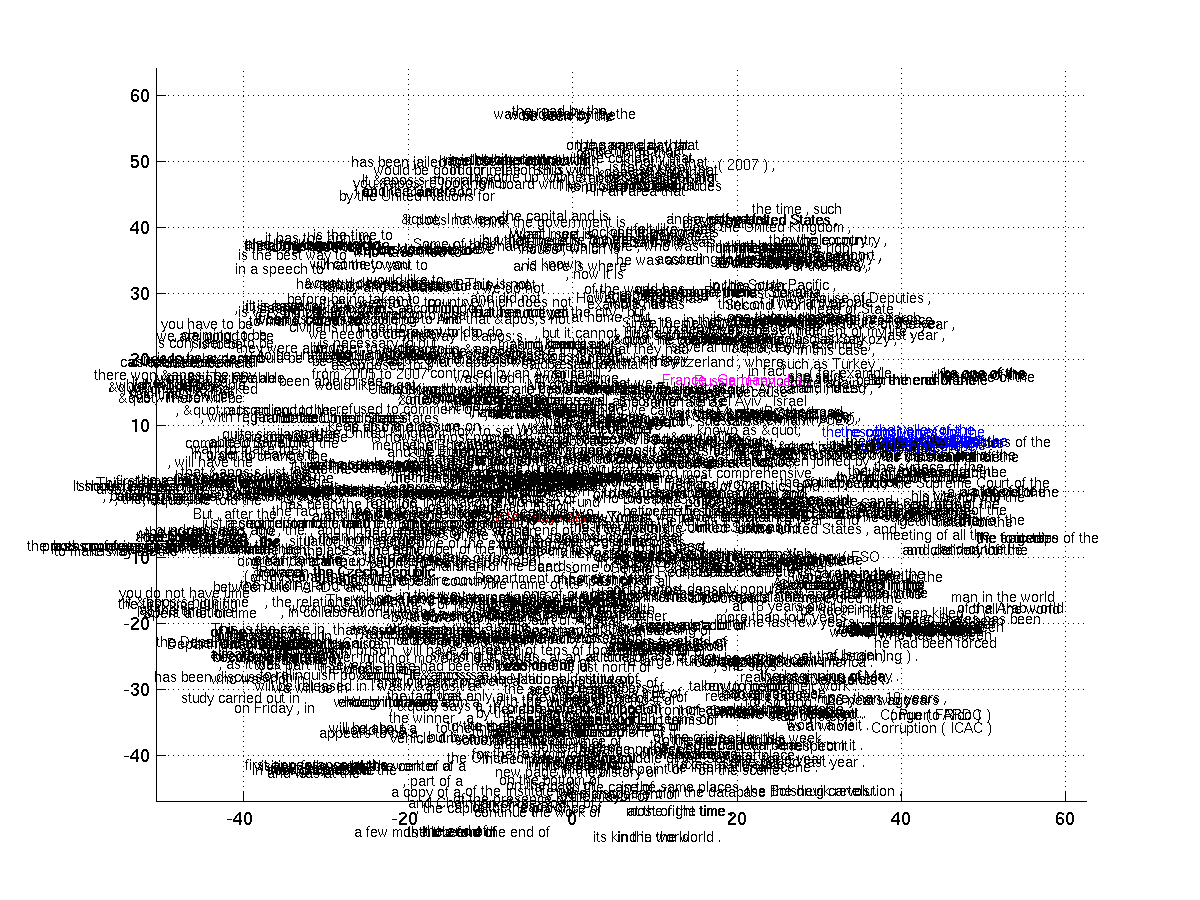
\includegraphics[width=0.99\textwidth]{phrase_all.png}
    \end{minipage}
    \begin{minipage}{0.75\textwidth}
        \centering
        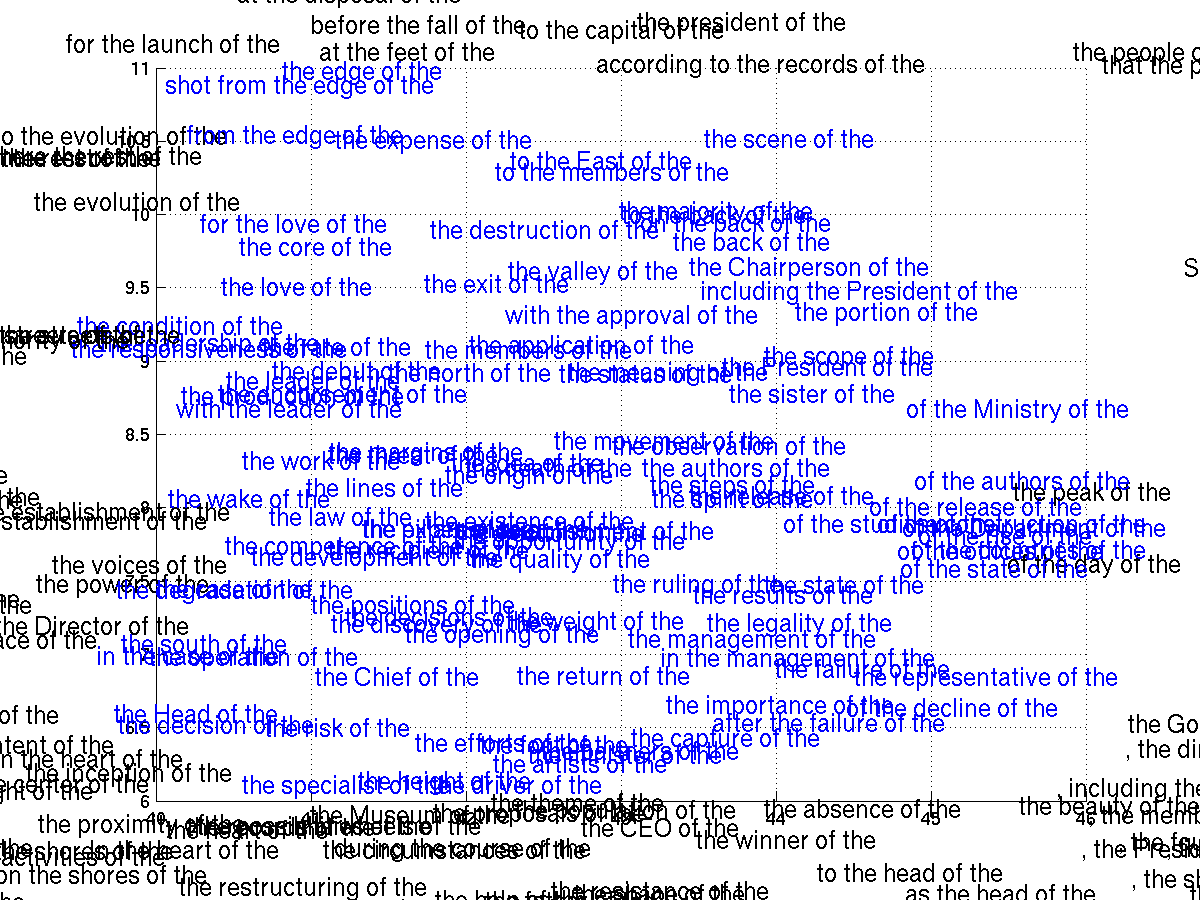
\includegraphics[width=0.99\textwidth]{phrase_zoom1.png}
    \end{minipage}
    \\
    \begin{minipage}{0.75\textwidth}
        \centering
        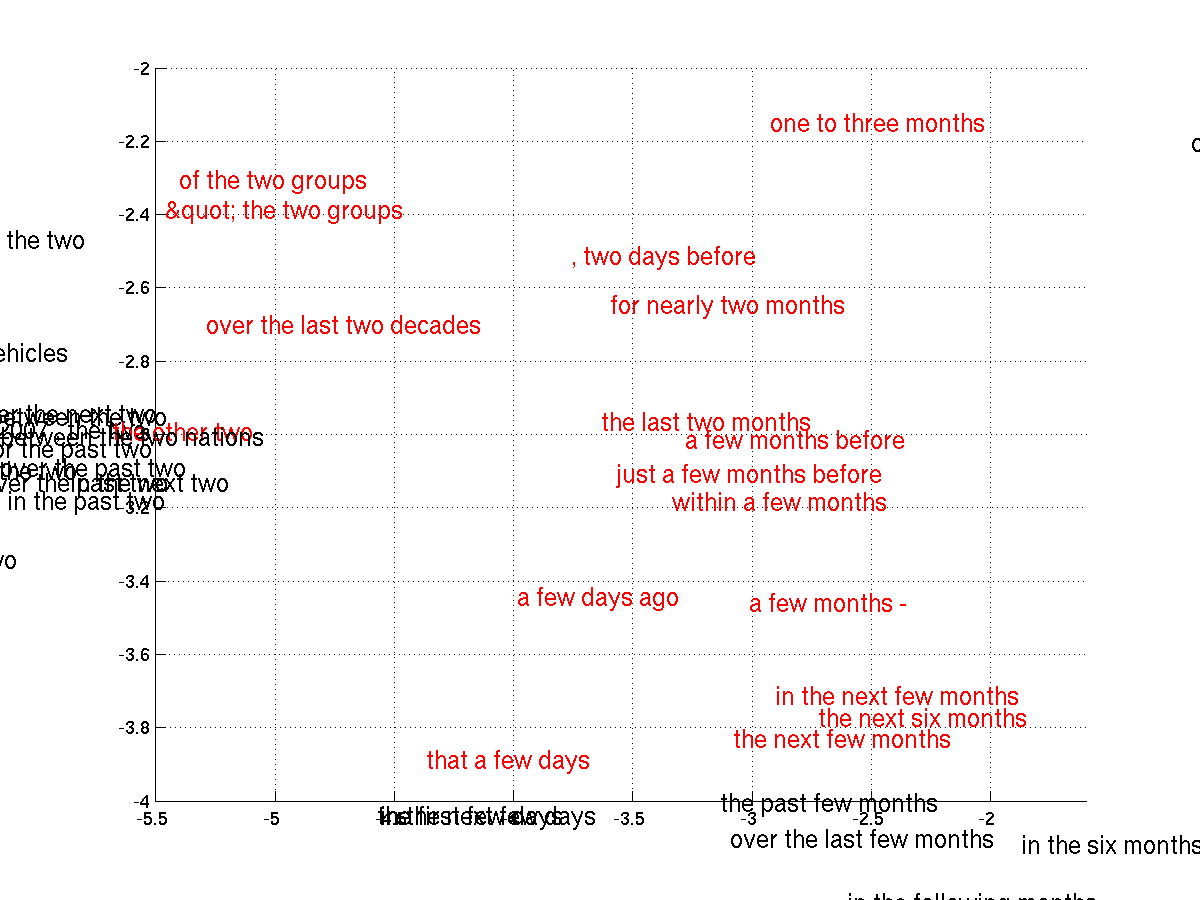
\includegraphics[width=0.99\textwidth]{phrase_zoom2.png}
    \end{minipage}
    \begin{minipage}{0.75\textwidth}
        \centering
        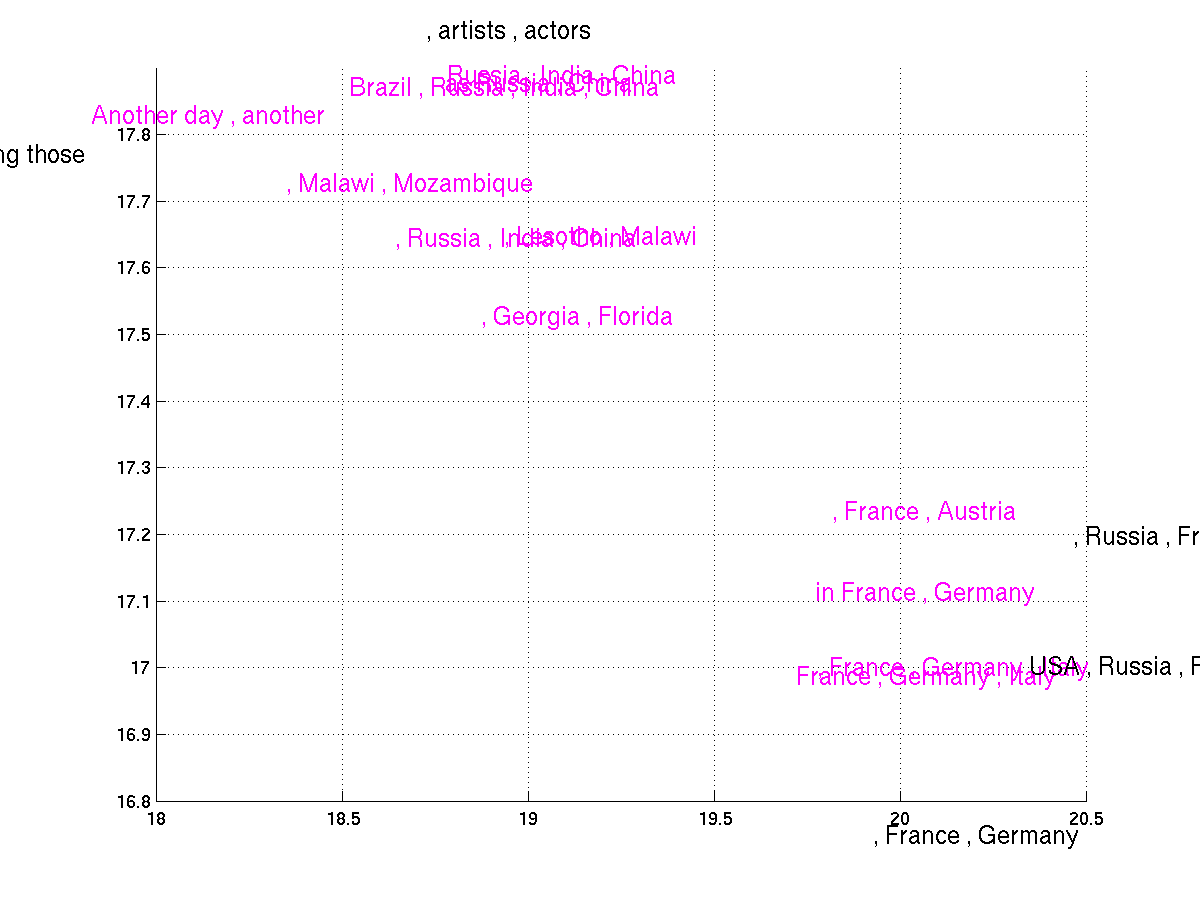
\includegraphics[width=0.99\textwidth]{phrase_zoom3.png}
    \end{minipage}
    \caption{2--D embedding of the learned phrase representation. The top left
    one shows the full representation space (1000 randomly selected points),
while the other three figures show the zoomed-in view of specific regions
(color--coded).} 
\end{figure*}
\end{landscape}



\end{document}
